\newpage
\chapter{RESULTADOS}

\par Neste capítulo serão apresentados os resultados e análises obtidos nos estudos dos dados. E para verificação dos algoritmos e dos dados o arquivo encontra-se no \emph{site} \emph{Github} no \emph{link}: https://github.com/nata27junior/Dataframe-Tg-dados.



\section{Resultados obtidos com Distância Euclidiana}
\par Com as funções descritas nas figuras \ref{dist_eu_py} e \ref{dist_eu_pynumpy}, e aplicando-as  nos dados  foram obtidos os seguintes resultados:

\begin{figure}[ht]
	\caption{\textbf{Aplicação Distância Euclidiana nos meses de Março e Abril de 2018}}
	\centering
		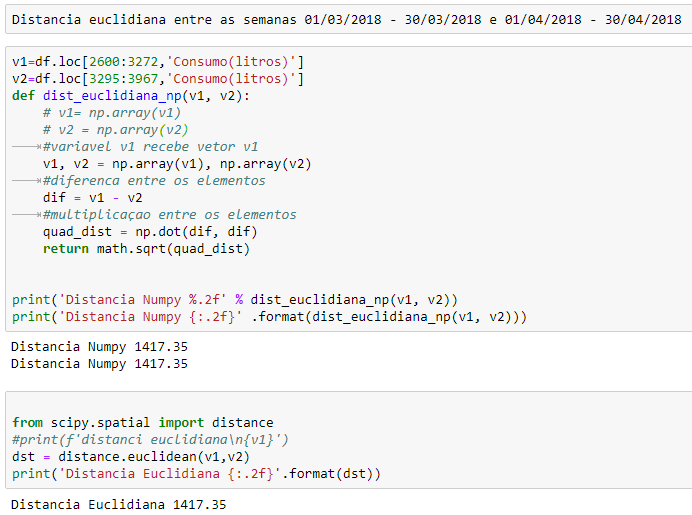
\includegraphics[width=\textwidth,height=\textheight , keepaspectratio]{figuras/distanciaeuclidiana01-03-2018-30-03-2018-01-04-18-30-04-18}
		\label{dist_Marco_Abril}
	%\fonte{\cite{fayyad1996data}}
\end{figure}
\par Com as funções de Distância Euclidiana, aplicadas nos dados relativos há dois meses, março de 2018 e abril de 2018, foi obtido o seguinte resultado de  $\approx$ 1417, observa-se isso na figura \ref{dist_Marco_Abril}.  Relembrando que distância euclidiana é uma das medidas de dissimilaridade entre comunidades mais utilizadas na prática. E quanto menor o valor da distância euclidiana entre os dados, mais próximos os pontos se apresentam, logo, quanto menor a distância entre os pontos, maior a eficiência do procedimento.

\begin{figure}[ht]
	\caption{\textbf{Gráfico de comparação dos meses de março e abril de 2018 com a Distância Euclidiana}}
	\centering
		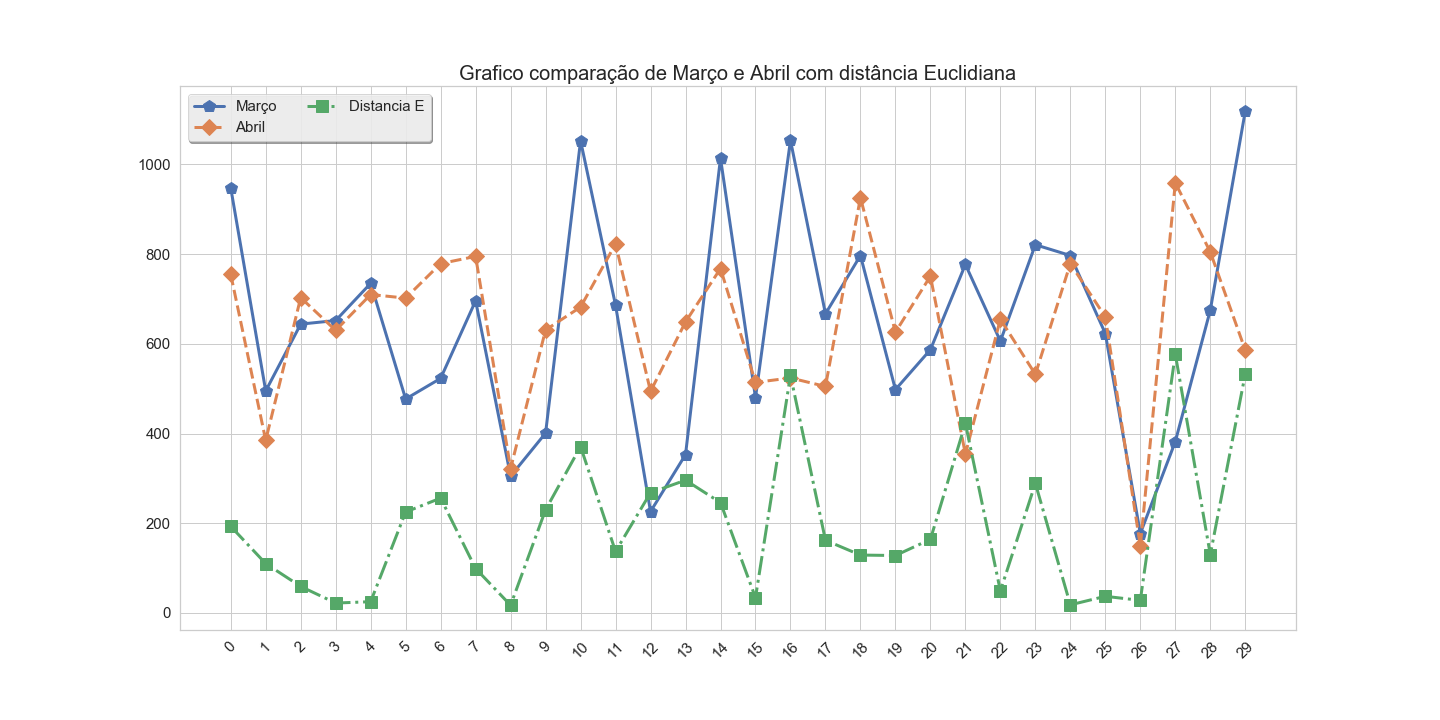
\includegraphics[width=\textwidth,height=\textheight , keepaspectratio]{figuras/ComparacaodeMarcoeAbrilcomdistanciaEuclidiana}
		\label{graf_dist_Marco_Abril}
	%\fonte{\cite{fayyad1996data}}
\end{figure}
\par Nesse gráfico, da figura \ref{graf_dist_Marco_Abril}, foi aplicada a função da Distância Euclidiana no consumo diário nos meses de março e abril de 2018, aplicada ponto a ponto, e notando se que em alguns dias o consumo diário dos meses foi quase semelhante onde os resultados da função da Distância Euclidiana quase se aproxima a zero. 

\begin{figure}[ht]
	\caption{\textbf{Aplicação da Distancia Euclidiana entre duas semanas setembro de 2017}}
	\centering
		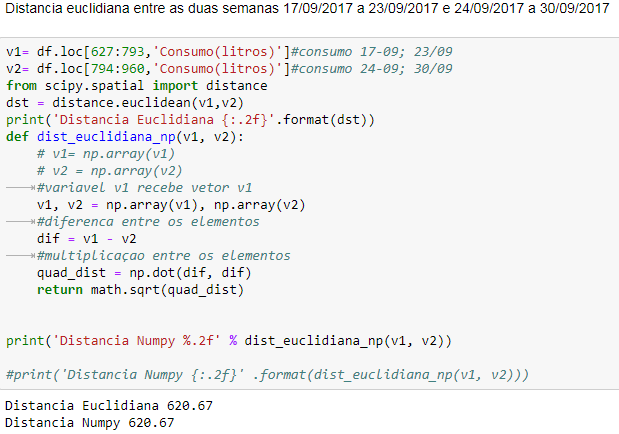
\includegraphics[width=\textwidth,height=\textheight , keepaspectratio]{figuras/distanciaeuclidiana17-09a23-09e24-09a30-09}
		\label{dist_duas_set}
	%\fonte{\cite{fayyad1996data}}
\end{figure}

\par Executando as funções de Distância Euclidiana entre duas semanas, de 17 de setembro a 23 de setembro e 24 de setembro a 30 de setembro, obteve-se o resultado de  $\approx$ 620. Mas uma vez, o resultado obtido não foi mais próximo de zero, como se observa na figura  \ref{dist_duas_set}.

\begin{figure}[ht]
	\caption{\textbf{Gráfico de comparação entre duas semanas com a Distância Euclidiana}}
	\centering
		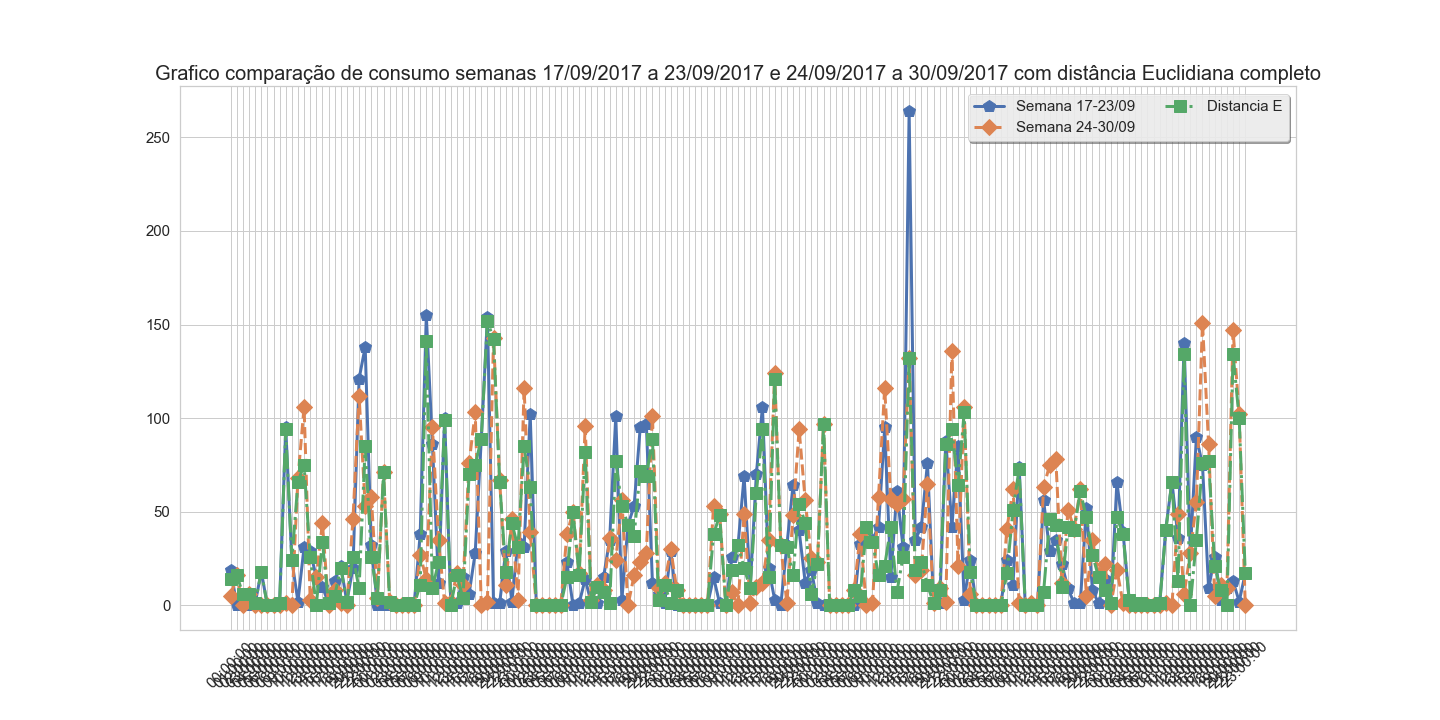
\includegraphics[width=\textwidth,height=\textheight , keepaspectratio]{figuras/Comparacaodesemanas17a23-09e24a30-09comdistanciacompleto}
		\label{dist_duas_set_comp}
	%\fonte{\cite{fayyad1996data}}
\end{figure}

\begin{figure}[ht]
	\caption{\textbf{Gráfico de comparação entre duas semanas com a Distância Euclidianas Detalhadas}}
	\centering
		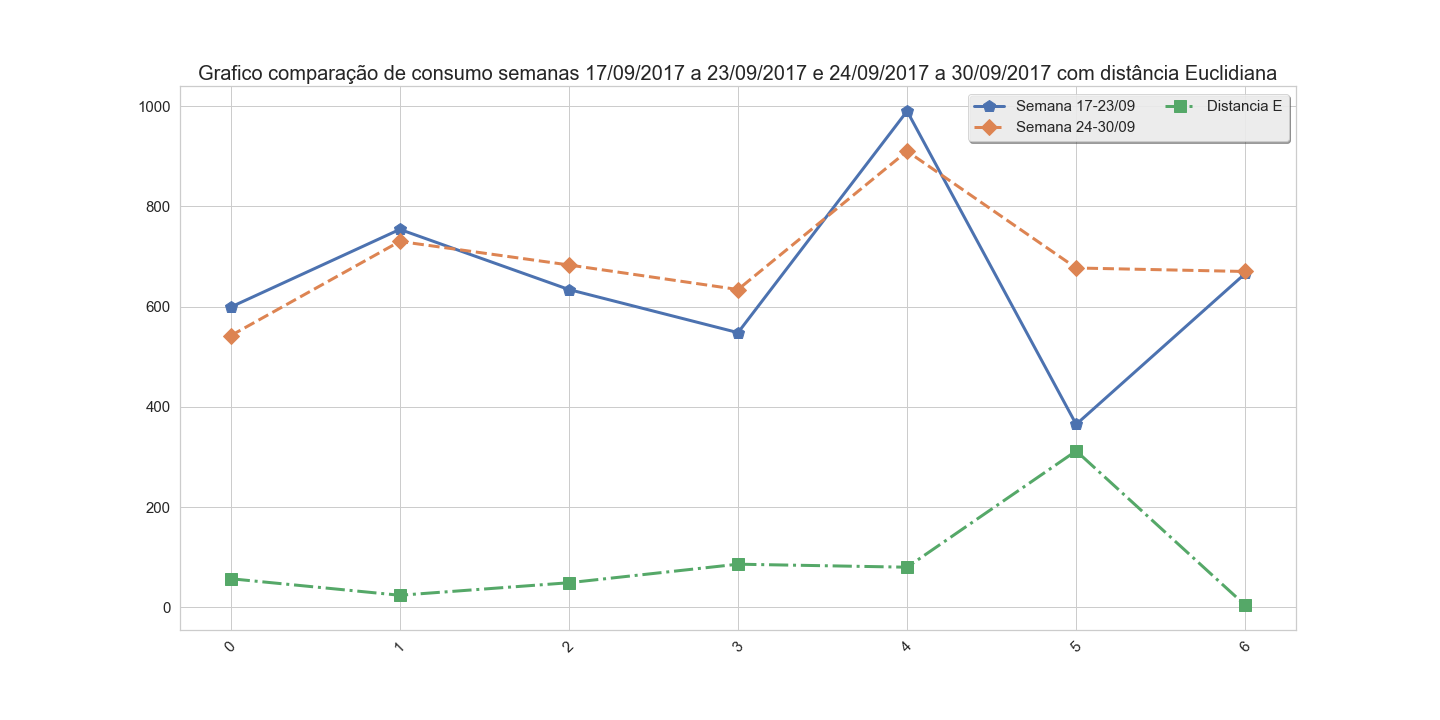
\includegraphics[width=\textwidth,height=\textheight , keepaspectratio]{figuras/Comparacaodesemanas17a23-09e24a30-09comdistancia}
		\label{dist_duas_set_deta}
	%\fonte{\cite{fayyad1996data}}
\end{figure}

\par No gráfico da figura \ref{dist_duas_set_comp} representa o consumo entre duas semanas de 17 de setembro a 23 de setembro e 24 de setembro a 30 de setembro, com a distância euclidiana aplicada ponto a ponto, mesmo com o gráfico com  os dados muito próximo pode verificar que há pontos onde o resultado da função aproximou de zero . E pode conferir com mais detalhes no gráfico da figura \ref{dist_duas_set_deta}, onde foi aplicada a função no consumo diário, observando que o consumo nos dias foram bem semelhante e o resultado da função foi bem próximo de zero. 

\begin{figure}[ht]
	\caption{\textbf{Aplicação da Distancia Euclidiana entre os dias 09 e 16 de setembro de 2017}}
	\centering
		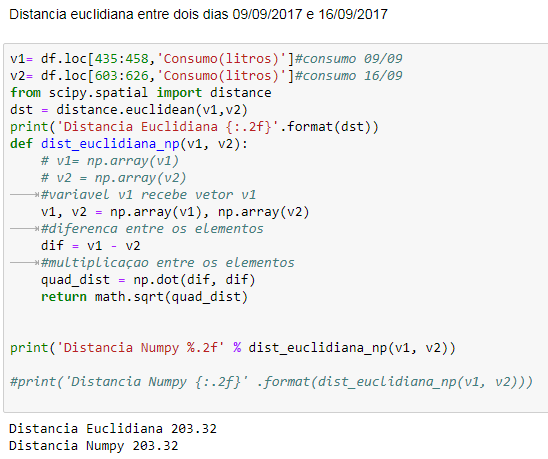
\includegraphics[scale=0.8 , keepaspectratio]{figuras/distanciaeuclidiana09-09-17e16-09-17}
		\label{dist_09e16_set_deta}
	%\fonte{\cite{fayyad1996data}}
\end{figure}

\par Executando as funções de Distância Euclidiana em dois dias, 09 e 16, do mês de setembro, dois sábados do mesmo mês, e obteve-se o resultado de  $\approx $203. Mas uma vez, o resultado obtido não sendo mais próximo de zero (0), como se observa na figura \ref{dist_09e16_set_deta}. 

\begin{figure}[ht]
	\caption{\textbf{Gráfico de comparação entre os dias 09 e 16 de setembro de 2017 com Distância Euclidiana}}
	\centering
		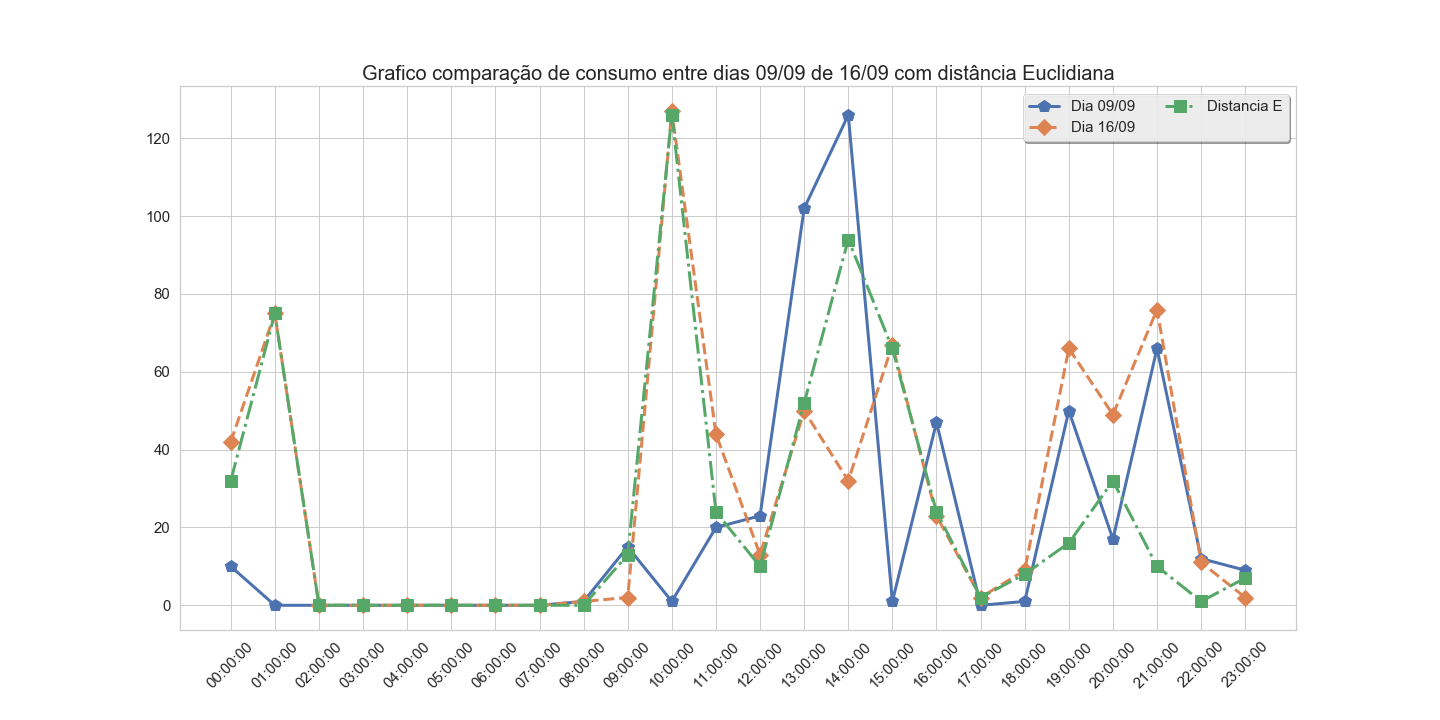
\includegraphics[width=\textwidth,height=\textheight , keepaspectratio]{figuras/Comparacaodedias09-09e16-09comdistancia}
		\label{graf_dist_09e16_set_deta}
	%\fonte{\cite{fayyad1996data}}
\end{figure}
\par O Gráfico da figura \ref{graf_dist_09e16_set_deta} representa o consumo entre dois dias, 09 de setembro e 16 de setembro, dois sábados do mesmo mês,  aplicada a função da Distância ponto a ponto, observa que no período onde não houve consumo os resultados foram próximos a zero, e em alguns pontos onde teve consumo o resultado da função também se aproximou de zero sendo um comportamento do consumo muito parecido.


\section{Resultados obtidos com a Função para plotagem de gráfico }
\par Com a função de plotagem de gráfico que foi discriminar na figura \ref{codigo_plotagem}, podemos verificar as seguintes situações. 

\begin{figure}[ht]
	\caption{\textbf{Gráfico de comparação entre Domingos}}
	\centering
		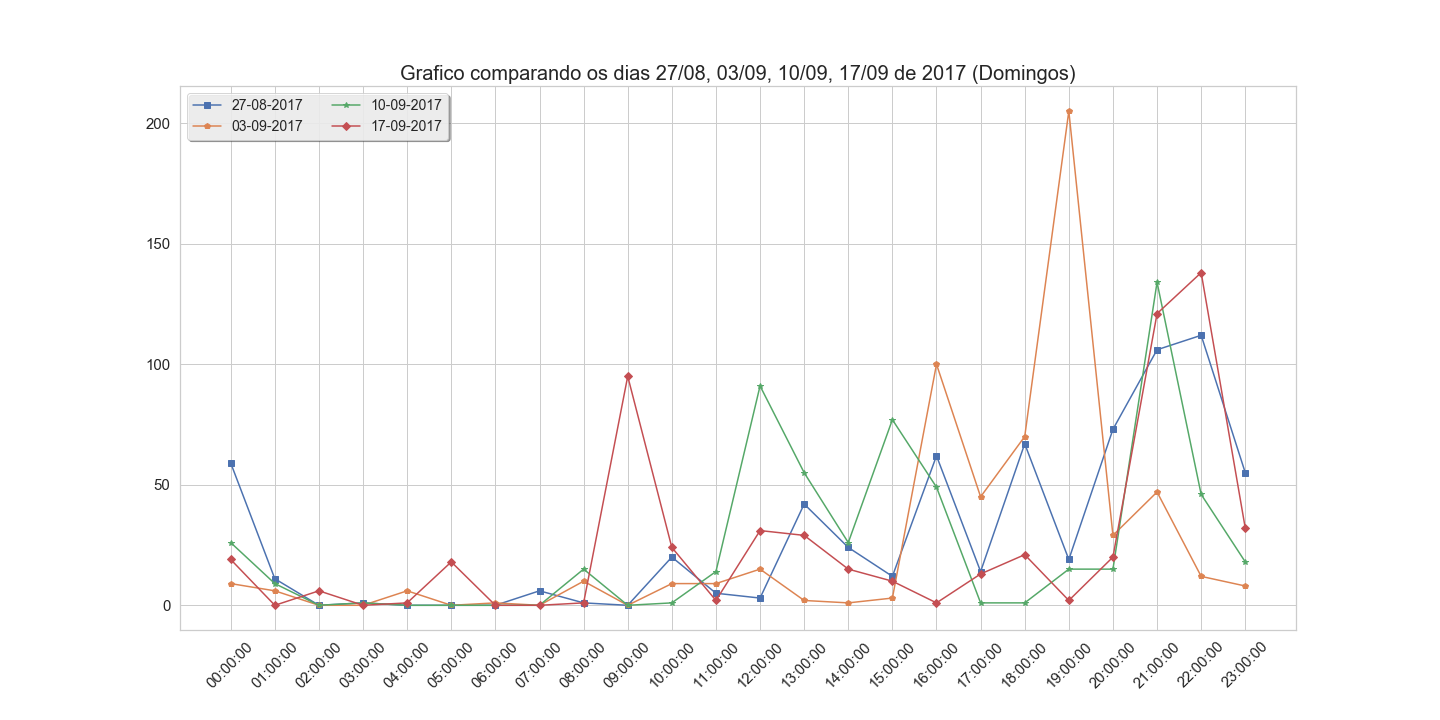
\includegraphics[width=\textwidth,height=\textheight , keepaspectratio]{figuras/Graficocomparandoosdias27-08,03-09,10-09,17-09de2017(Domingos)}
		\label{graf_dom}
	%\fonte{\cite{fayyad1996data}}
\end{figure}

\par No gráfico da figura \ref{graf_dom}, é possível comparar os dados das seguintes datas, 27/08/2017, 03/09/2017, 10/09/2017, 17/09/2017, que são Domingos, primeiramente é observado que há um consumo semelhante entre os dias. Mas nos períodos da madrugada há um baixo consumo de água onde pode verificar  que não há vazamentos. E onde ocorrem os picos de consumo que observando mas a fundo pode se afirmar que não é um vazamentos, pois se fosse vazamento o consumo seria mais constante.  

\begin{figure}[ht]
	\caption{\textbf{Gráfico de comparação entre Segundas-Feiras}}
	\centering
		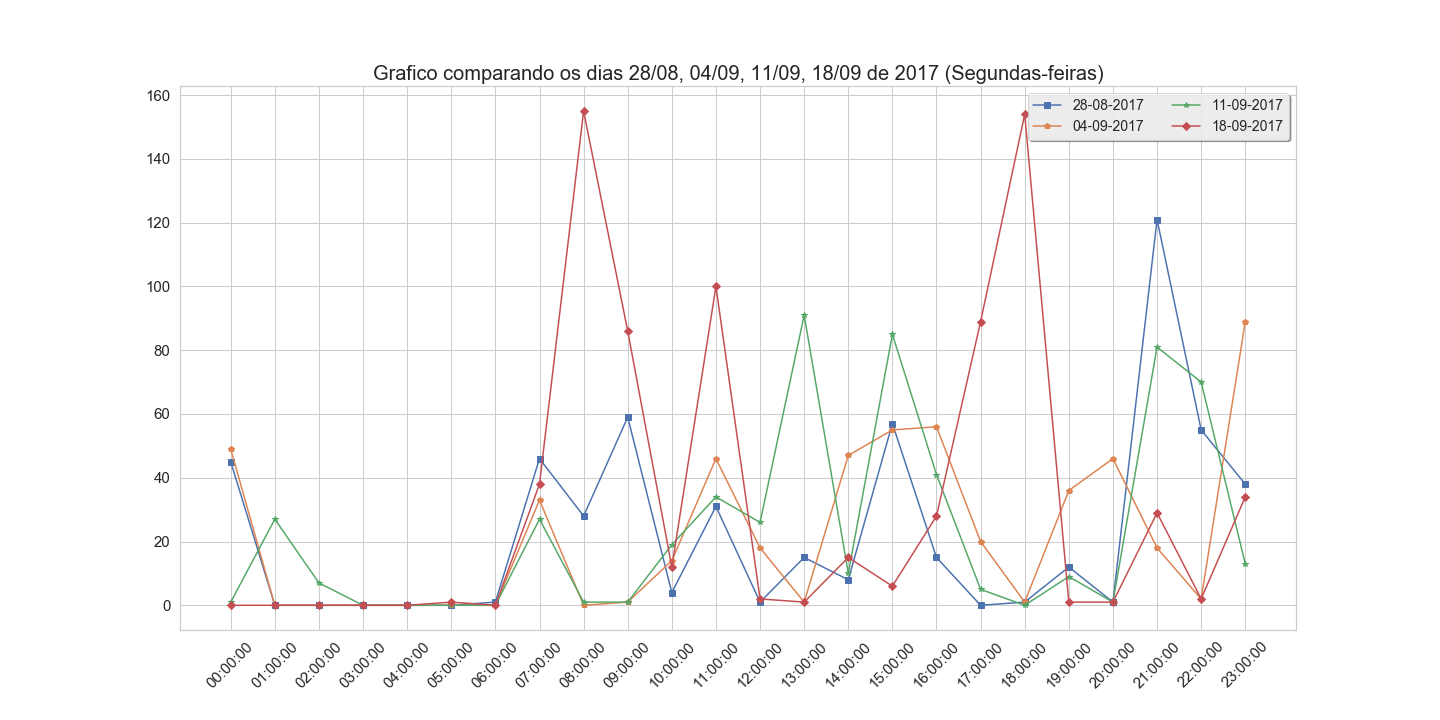
\includegraphics[width=\textwidth,height=\textheight , keepaspectratio]{figuras/Graficocomparandoosdias28-08,04-09,11-09,18-09de2017(Segundas-feiras)}
		\label{graf_seg}
	%\fonte{\cite{fayyad1996data}}
\end{figure}

\par No gráfico da figura \ref{graf_seg}, foi aplicada a função de plotagem com os dados das datas, 28/08/2017, 04/09/2017, 11/09/2017, 18/09/2017, que são segundas-feiras, obteve essa comparação dos dados, e que há um consumo semelhante.Mas nos períodos da madrugada há um baixo consumo de água onde pode verificar  que não há vazamentos. E onde ocorrem os picos de consumo que observando mas a fundo pode se afirmar que não é um vazamentos, pois se fosse vazamento o consumo seria mais constante.    

\begin{figure}[ht]
	\caption{\textbf{Gráfico de comparação entre Terças-Feiras}}
	\centering
		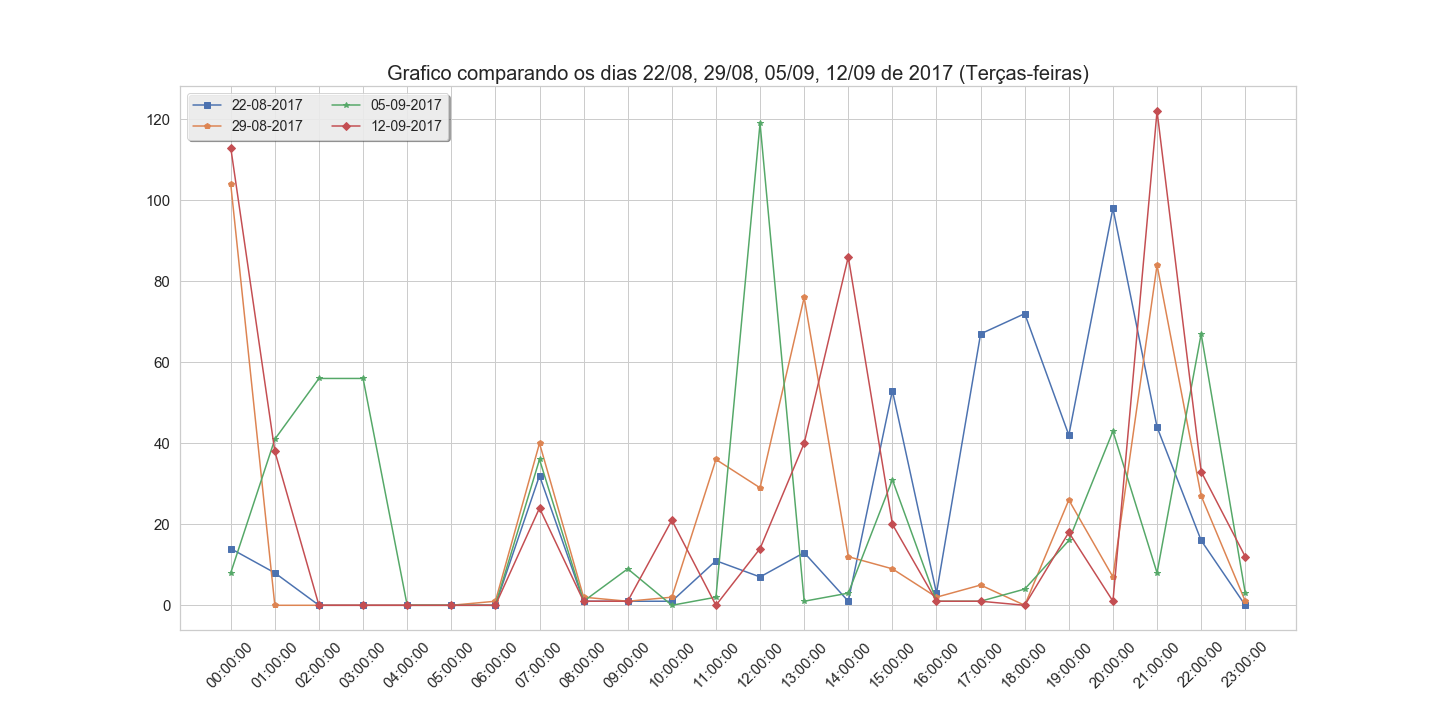
\includegraphics[width=\textwidth,height=\textheight , keepaspectratio]{figuras/Graficocomparandoosdias22-08,29-08,05-09,12-09de2017(Tercas-feiras)}
		\label{graf_ter}
	%\fonte{\cite{fayyad1996data}}
\end{figure}

\par No gráfico da figura \ref{graf_ter}, foi aplicada a função de plotagem com os dados das datas, 22/08/2017, 29/08/2017, 05/09/2017, 12/09/2017, que são terças-feiras, obteve essa comparação dos dados, e que há um consumo semelhante. Mas nos períodos da madrugada há um baixo consumo de água onde pode verificar  que não há vazamentos. E onde ocorrem os picos de consumo que observando mas a fundo pode se afirmar que não é um vazamentos, pois se fosse vazamento o consumo seria mais constante.   

\begin{figure}[ht]
	\caption{\textbf{Gráfico de Comparação dos dados entre Quartas-feiras}}
	\centering
		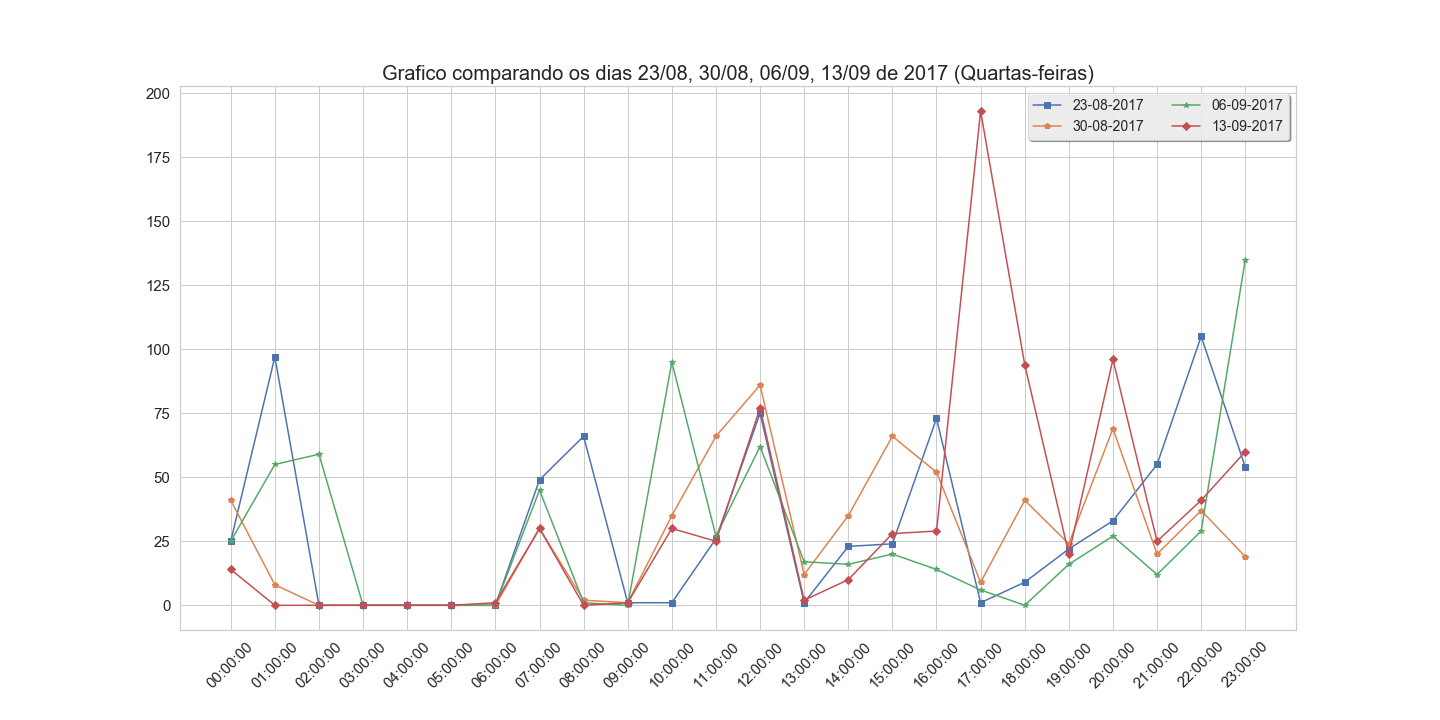
\includegraphics[width=\textwidth,height=\textheight , keepaspectratio]{figuras/Graficocomparandoosdias23-08,30-08,06-09,13-09de2017(Quartas-feiras)}
		\label{graf_quar}
	%\fonte{\cite{fayyad1996data}}
\end{figure}
\par No gráfico da figura \ref{graf_quar}, foi aplicada a função de plotagem com os dados das datas, 23/08/2017, 30/08/2017, 06/09/2017, 13/09/2017, que são quartas-feiras, obteve essa comparação dos dados, nota-se e que há um consumo semelhante. Mas nos períodos da madrugada há um baixo consumo de água onde se pode notar que não há vazamentos. E onde ocorrem os picos de consumo que observando, mas a fundo pode se afirmar que nesses picos não é um vazamentos, pois se fosse vazamento o consumo seria mais constante.  
%\begin{figure}[htb]
\begin{figure}[ht]
	\caption{\textbf{Gráfico de Comparação dos dados entre Quintas-feiras}}
	\centering
		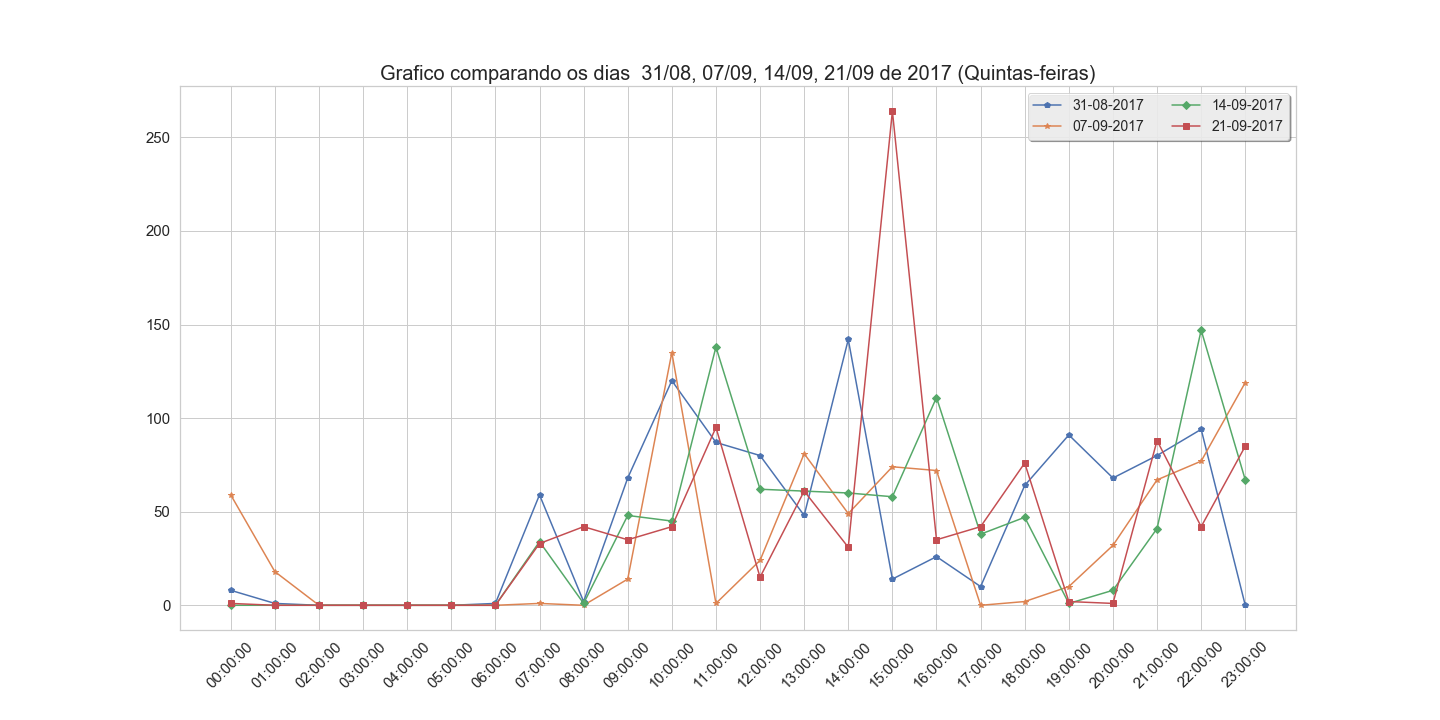
\includegraphics[width=\textwidth,height=\textheight , keepaspectratio]{figuras/Graficocomparandoosdias31-08,07-09,14-09,21-09de2017(Quintas-feiras)}
		\label{graf_qui}
	%\fonte{\cite{fayyad1996data}}
\end{figure}

\par No gráfico da figura \ref{graf_qui}, foi aplicada a função de plotagem com os dados das datas, 31/08/2017, 07/09/2017, 14/09/2017, 21/09/2017, que são quintas-feiras, obteve essa comparação dos dados, nota-se que há um consumo semelhante. Mas nos períodos da madrugada há um baixo consumo de água onde se pode notar que não há vazamentos. E onde ocorrem os picos de consumo que observando, mas a fundo pode se afirmar que nesses picos não é um vazamentos, pois se fosse vazamento o consumo seria mais constante.  

\begin{figure}[ht]
	\caption{\textbf{Gráfico de Comparação dos dados entre Sextas-feiras}}
	\centering
		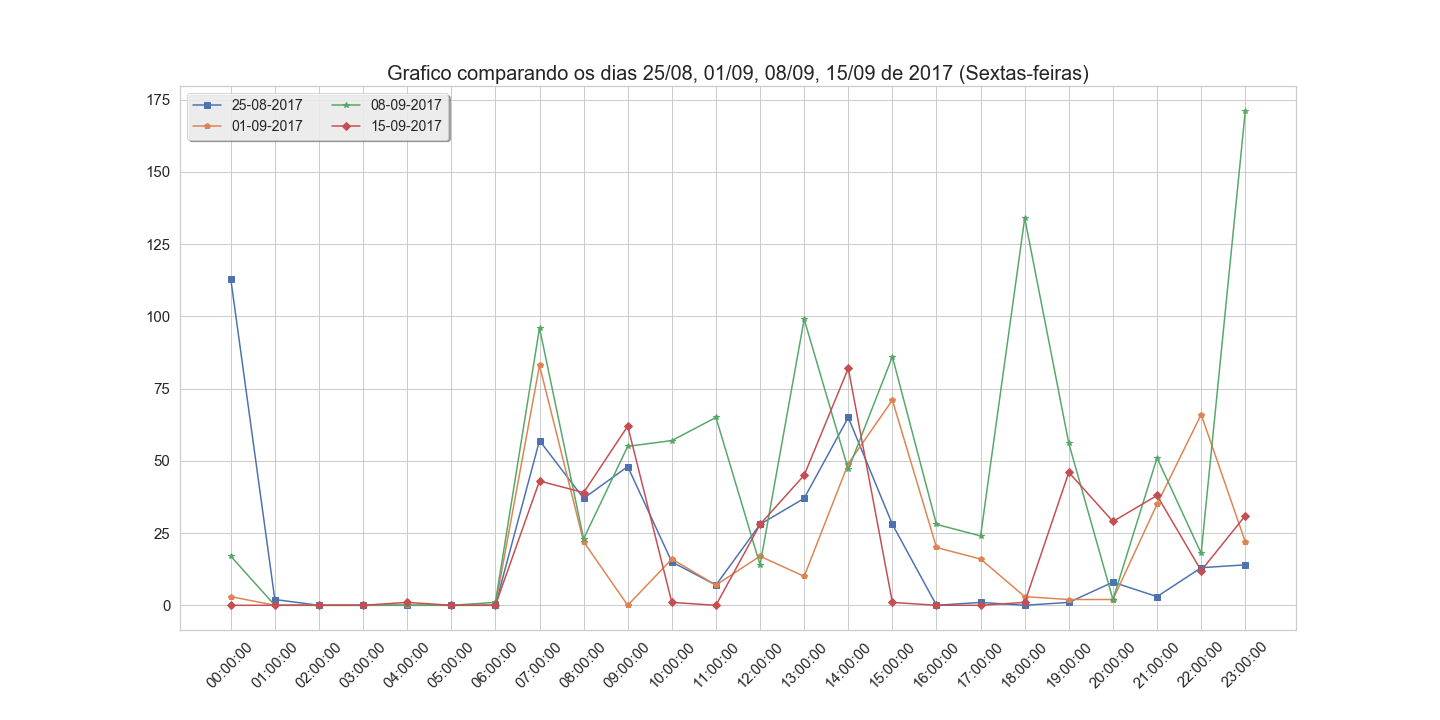
\includegraphics[width=\textwidth,height=\textheight , keepaspectratio]{figuras/Graficocomparandoosdias25-08,01-09,08-09,15-09de2017(Sextas-feiras)}
		\label{graf_sex}
	%\fonte{\cite{fayyad1996data}}
\end{figure}
\par No gráfico da figura \ref{graf_sex}, foi aplicada a função de plotagem com os dados das datas de 31/08, 07/09, 14/09 e 21/09/2017, que são sextas-feiras, obteve essa comparação dos dados, nota-se e que há um consumo semelhante. Mas nos períodos da madrugada há um baixo consumo de água onde se pode notar que não há vazamentos. E onde ocorrem os picos de consumo que observando, mas a fundo pode se afirmar que nesses picos não é um vazamentos, pois se fosse vazamento o consumo seria mais constante.  

\begin{figure}[ht]
	\caption{\textbf{Gráfico de Comparação dos dados entre Sábados}}
	\centering
		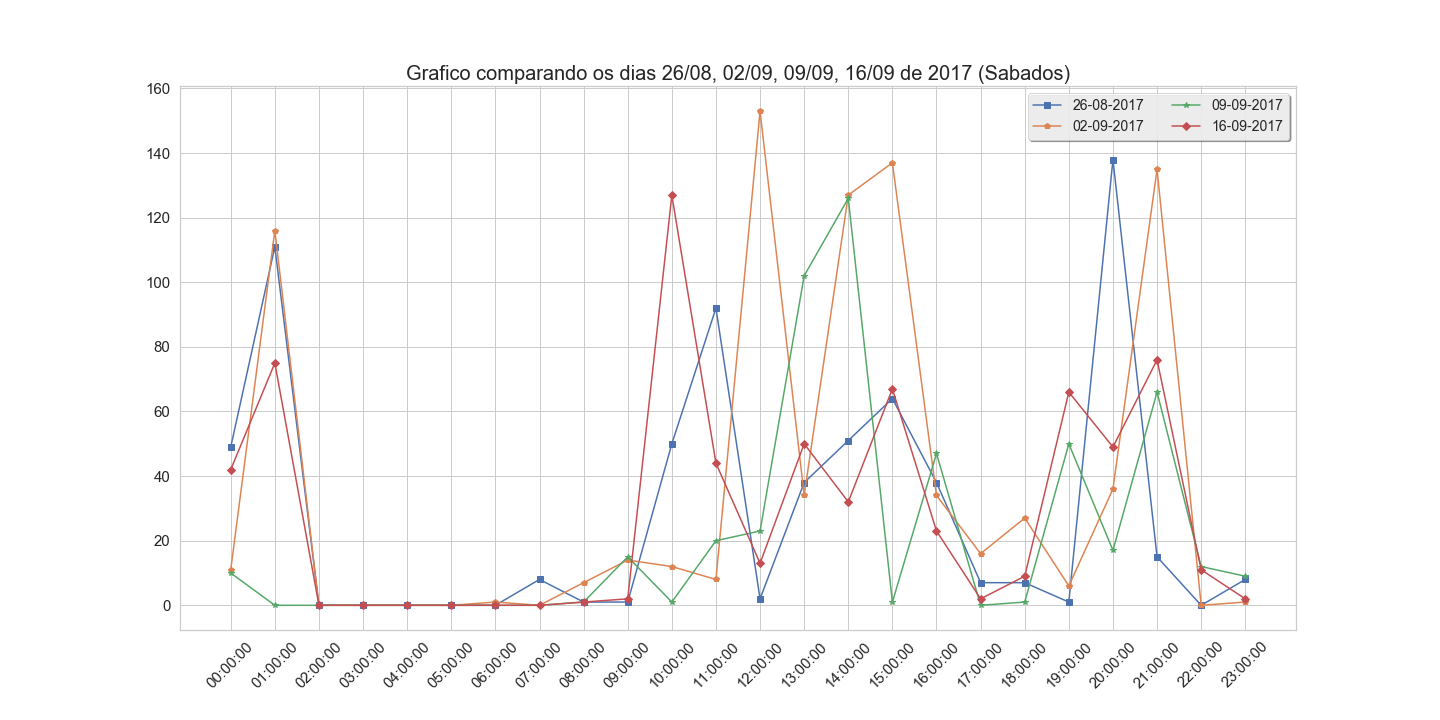
\includegraphics[width=\textwidth,height=\textheight , keepaspectratio]{figuras/Graficocomparandoosdias26-08,02-09,09-09,16-09de2017(Sabados)}
		\label{graf_sab}
	%\fonte{\cite{fayyad1996data}}
\end{figure}

\par No gráfico da figura \ref{graf_sab}, foi aplicada a função de plotagem com os dados das datas  de 26/08, 02/09, 09/09 e 16/09/2017, que são sábados, obteve essa comparação dos dados, nota-se e que há um consumo semelhante. Mas nos períodos da madrugada há um baixo consumo de água onde se pode notar que não há vazamentos. E onde ocorrem os picos de consumo que observando, mas a fundo pode se afirmar que nesses picos não é um vazamentos, pois se fosse vazamento o consumo seria mais constante.

\begin{figure}[ht]
	\caption{\textbf{Gráfico de comparação com diferença entre 03 a 09/09 e 10 a 16/09}}
	\centering
		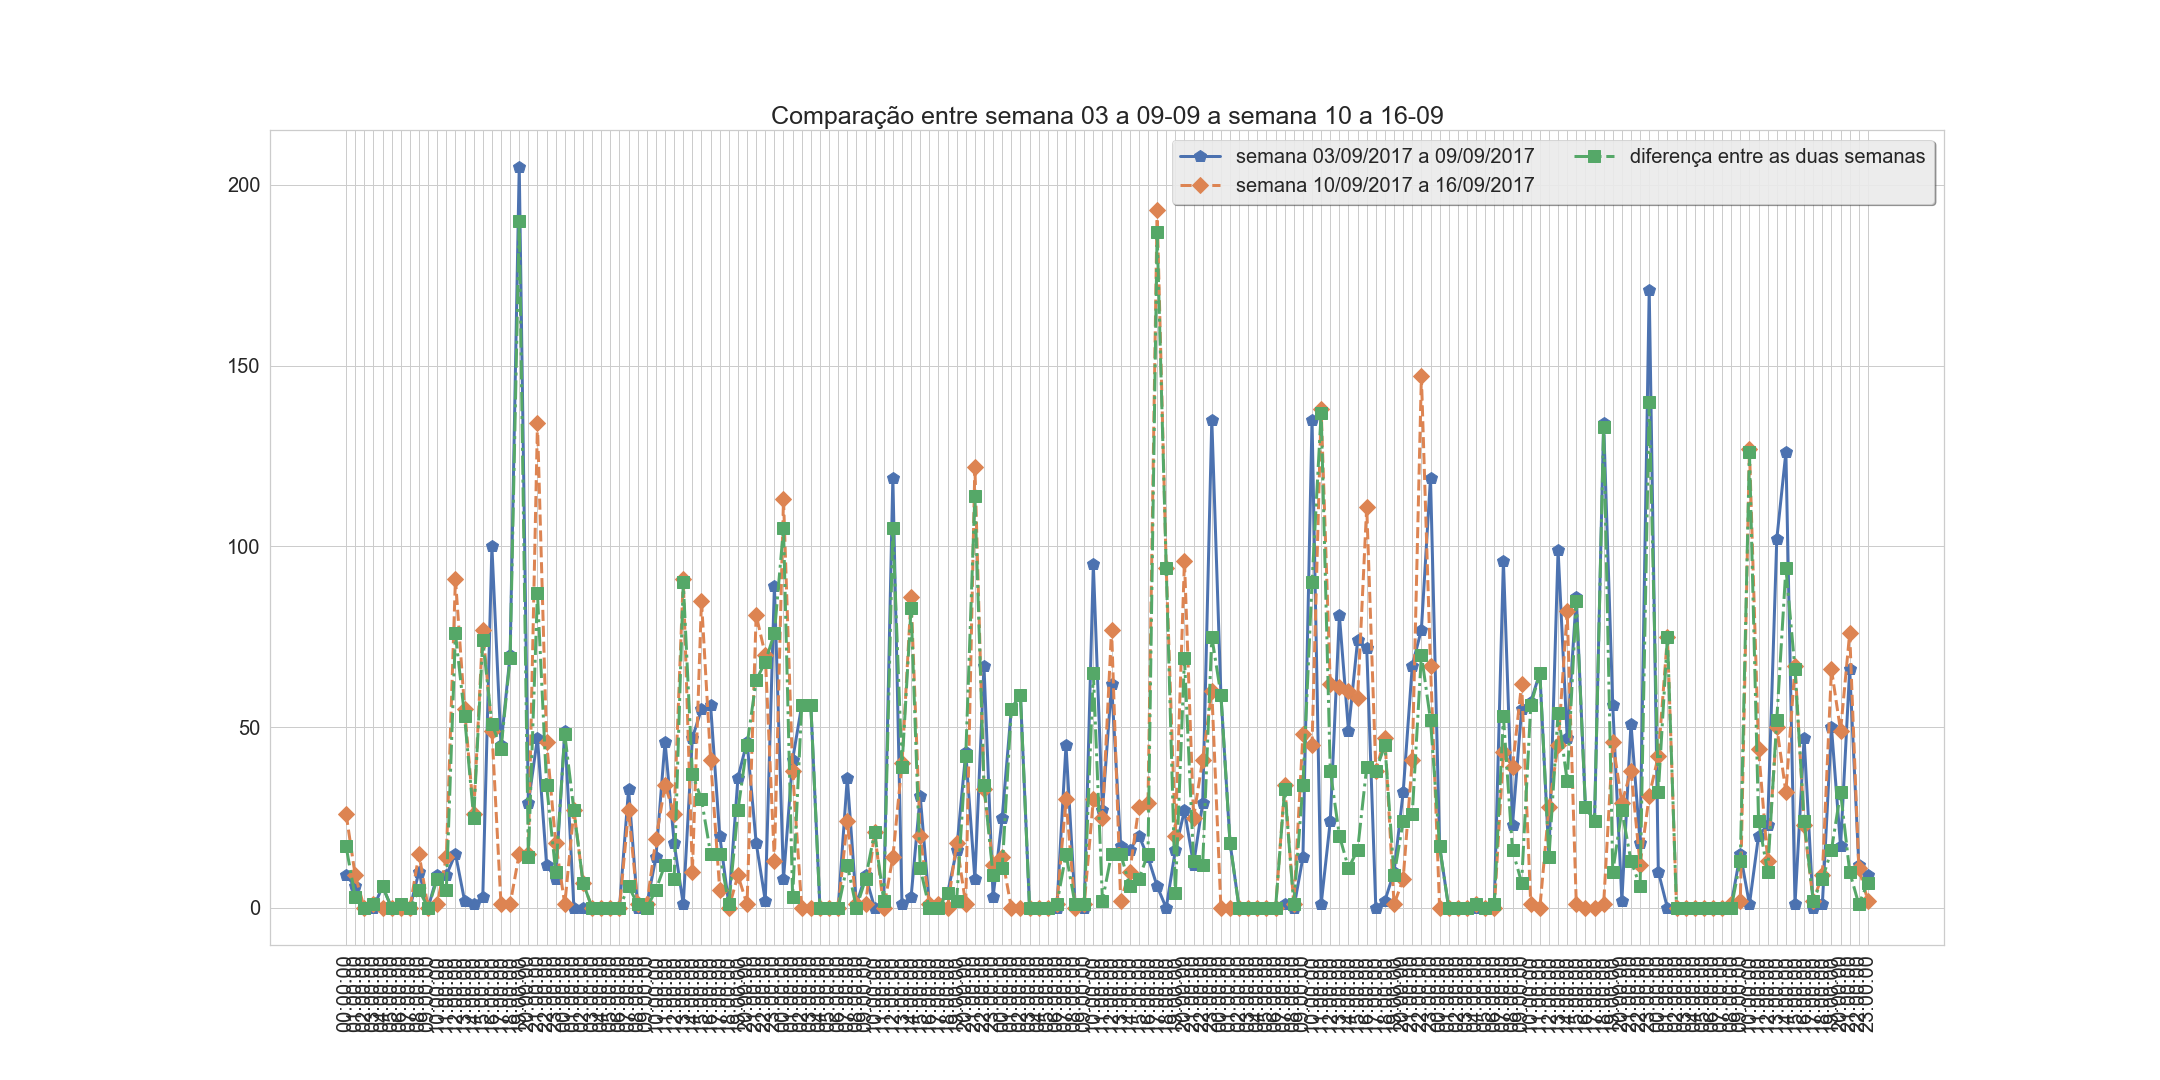
\includegraphics[width=\textwidth,height=\textheight , keepaspectratio]{figuras/comparacaoentresemana03a09-09asemana10a16-09}
		\label{graf_semana03a09}
	%\fonte{\cite{fayyad1996data}}
\end{figure}
\par Com o gráfico da figura \ref{graf_semana03a09}, trata-se da aplicação da função de plotagem fazendo uma comparação dos dados entre duas semanas. Uma semana é de 03 de setembro a 09 de setembro e outra semana é de 10 de setembro a 16 de setembro, e uma linha do gráfico se trata de diferença de consumo hora a hora entre essas duas semanas. Com os pontos muito próximos fica complicada a visualização dos pontos, mas há períodos onde não há consumo podendo afirmar que não houve vazamentos.

\begin{figure}[ht]
	\caption{\textbf{Gráfico detalha a comparação com diferença entre a 09/09 e  16/09}}
	\centering
		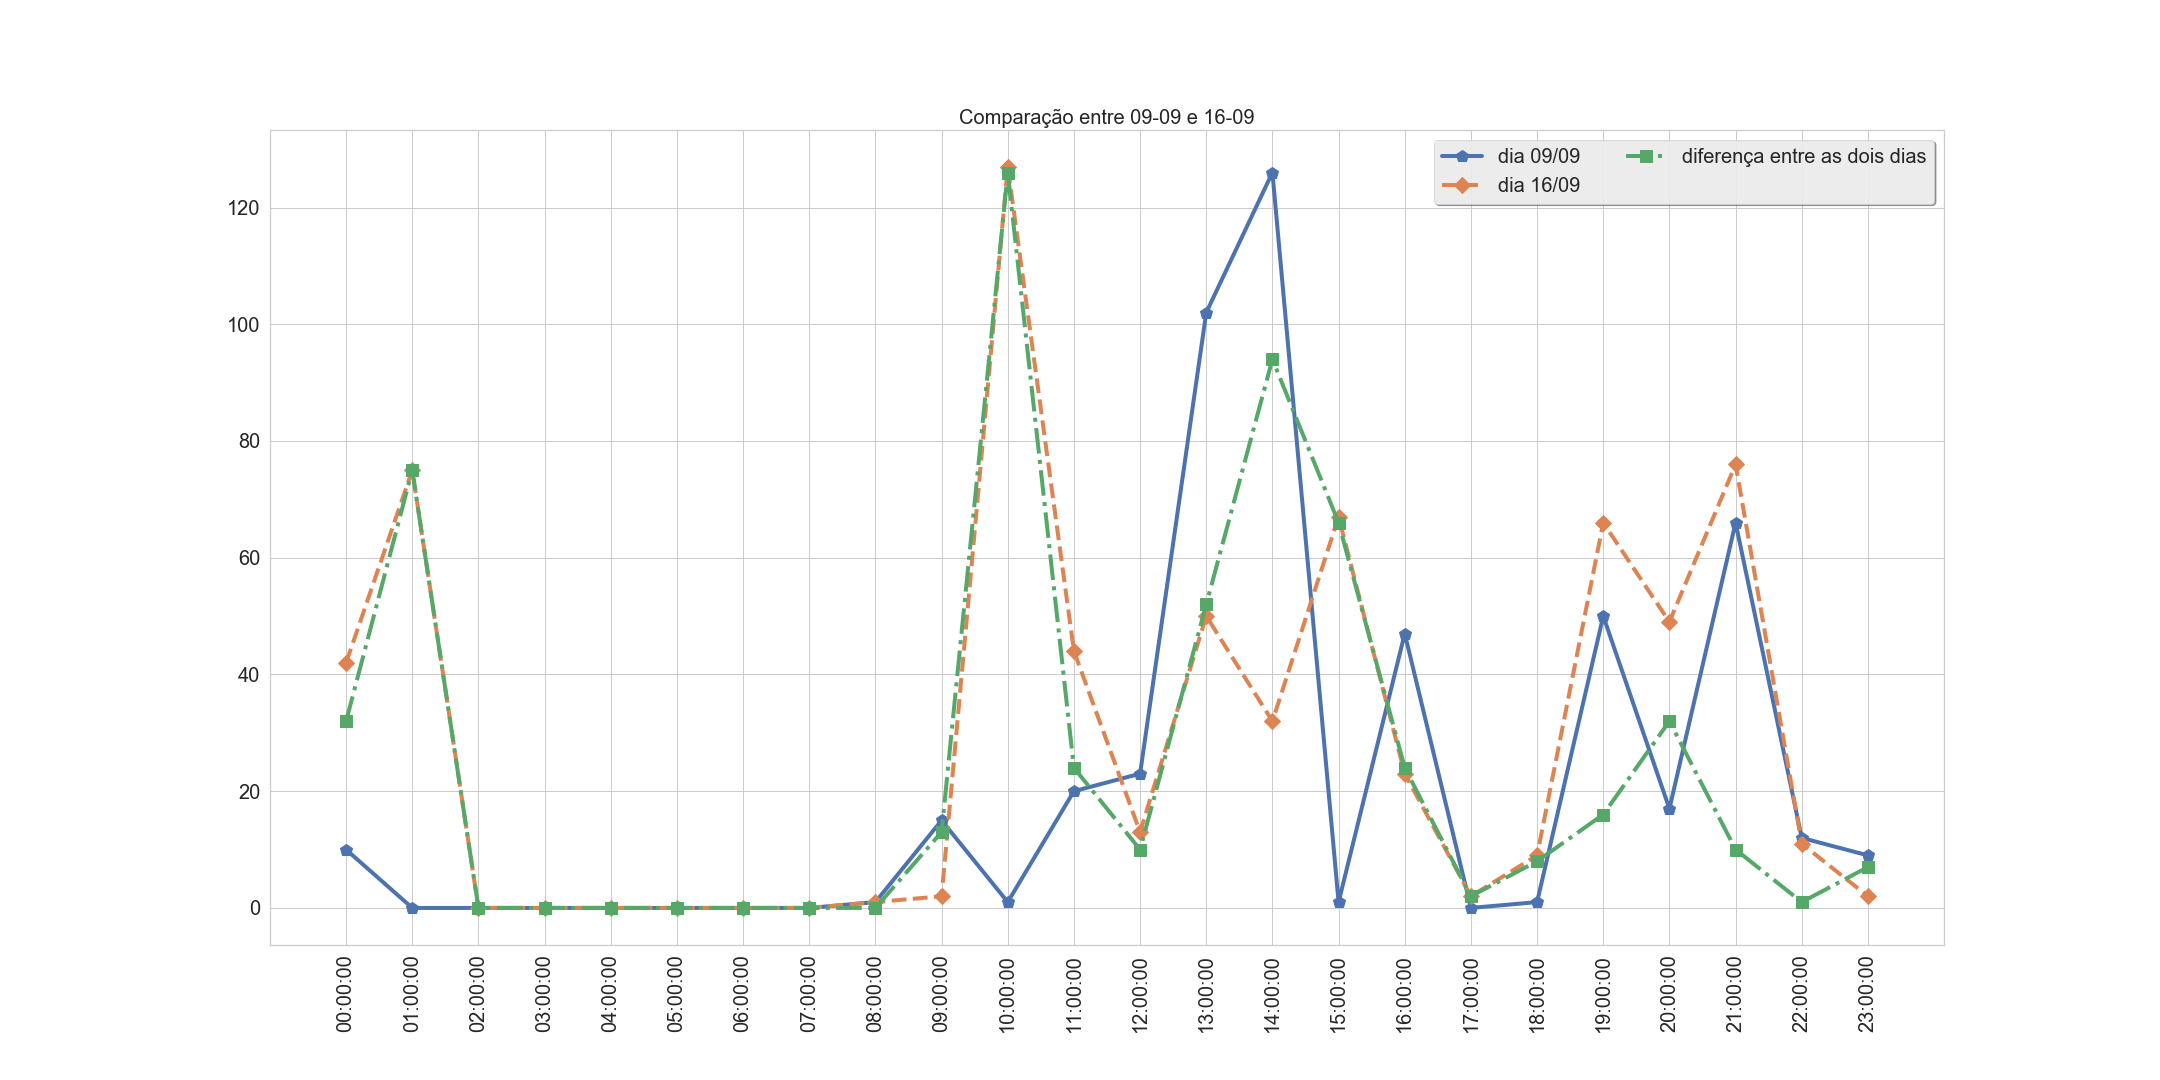
\includegraphics[width=\textwidth,height=\textheight , keepaspectratio]{figuras/zoomdacomparacaoentresemana03a09-09asemana10a16-09}
		\label{graf_det_semana03a09}
	%\fonte{\cite{fayyad1996data}}
\end{figure}
\par Com o gráfico da figura \ref{graf_det_semana03a09} trata-se da aplicação da função de plotagem nos dados fazendo uma comparação entre dois dias, com uma linha mostrando a diferença ponto a ponto, os dados utilizados para esse gráfico foi os dados dos dias 09 e 16 de setembro de 2017 e trata-se das últimas 24 horas podendo ver com mais detalhes as linhas que dos dias e a diferença dos dados. Nos horários da madrugada pode-se verificar que não há consumo de água.  

\begin{figure}[ht]
	\caption{\textbf{Figuras mostrando os dias com maior consumo de água}}
	\centering
		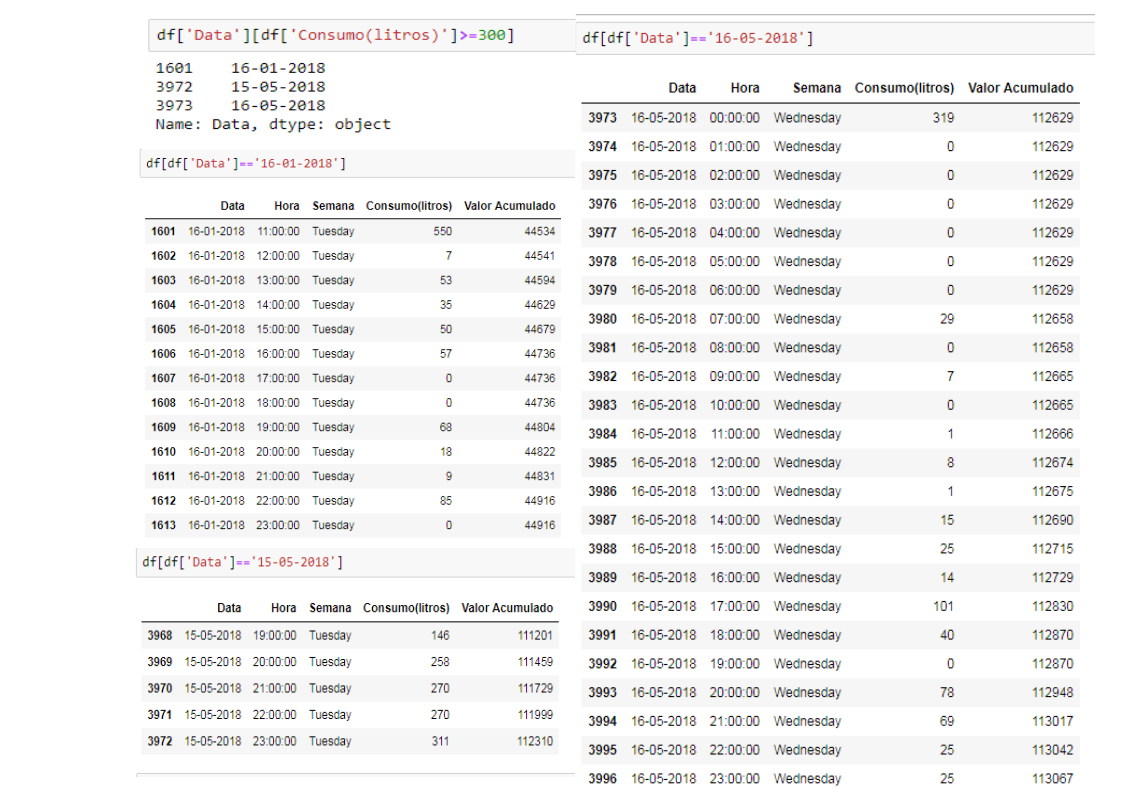
\includegraphics[width=\textwidth,height=\textheight , keepaspectratio]{figuras/datascommaiorconsumo2}
		\label{fig_maior_consumo}
	%\fonte{\cite{fayyad1996data}}
\end{figure}

\begin{figure}[ht]
	\caption{\textbf{Plotagem dos dados dos dias de maior consumo}}
	\centering
		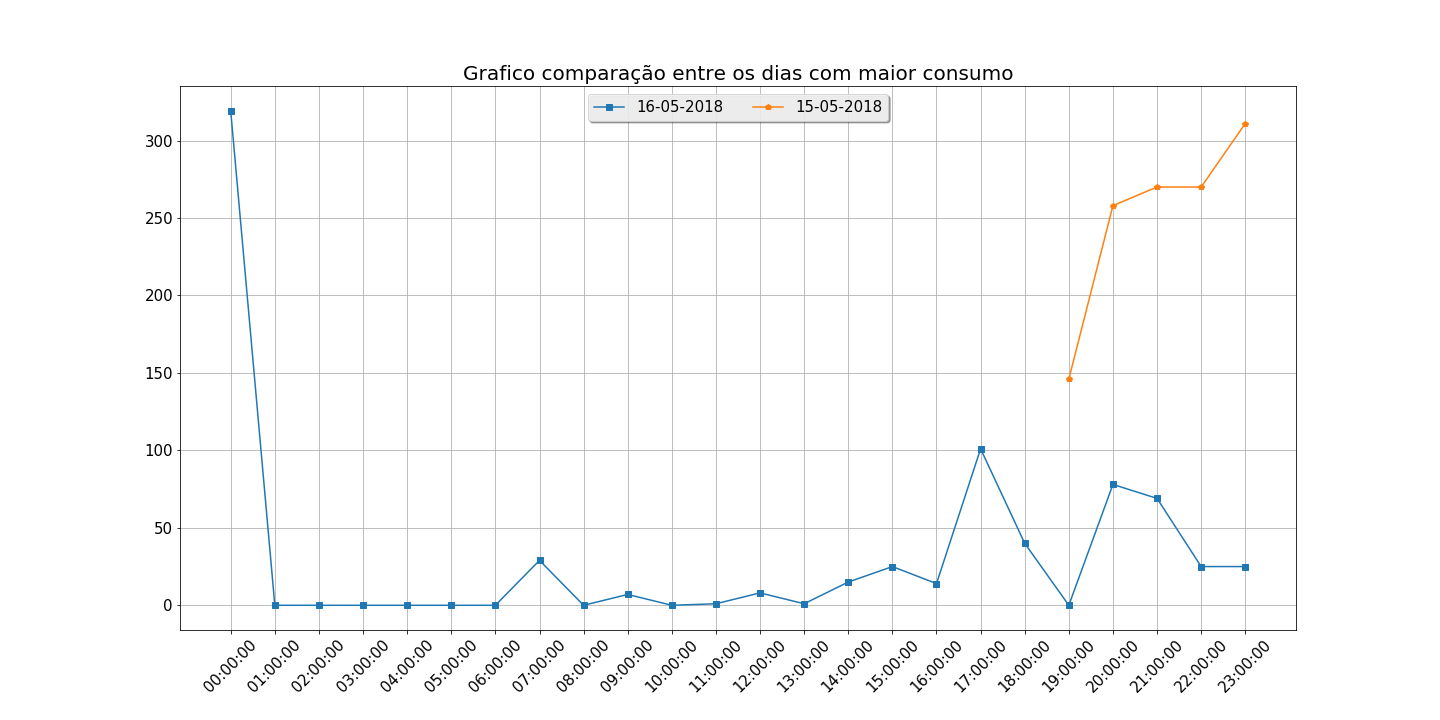
\includegraphics[width=\textwidth,height=\textheight , keepaspectratio]{figuras/comparacaoentreosdiascommaiorconsumo}
		\label{plot_maior_consumo}
	%\fonte{\cite{fayyad1996data}}
\end{figure}

\par Na figura \ref{fig_maior_consumo},  utiliza-se uma função especifica para mostrar os dias com maior consumo de água. Esses dias o consumo ultrapassa os 300 litro de água. Na figura \ref{plot_maior_consumo} uma plotagem que mostra os dias com maior consumo de água. Nota-se que no dia 15/05/2018 não tem os dados de consumo de todas as horas. O registro dos  dados é a partir das 19hs, não foi passada a informação se houve falha no equipamento para obtenção dos dados, ocasionando essa amostra com índice muito elevado de consumo. No dia 16/05/2018 há o registro de consumo após as 00hs, não se sabe se foi decorrente ao dia anterior que teve falha nos dados ou se realmente foi um consumo excessivo, mas como já observado nas horas da madrugada não há consumo de água, passa-se a ideia que no sistema não houve vazamento. O mesmo ocorre no  dia 16/01/2018 também se obteve um registro de dados elevado acima de 550 litros, como se pode notar a obtenção dos dados foi a partir das 11hs, então não se sabe se foi falha no sistema ou realmente teve um consumo elevado.

\begin{figure}[ht]
	\caption{\textbf{Gráfico com médias diárias de toda amostragem}}
	\centering
		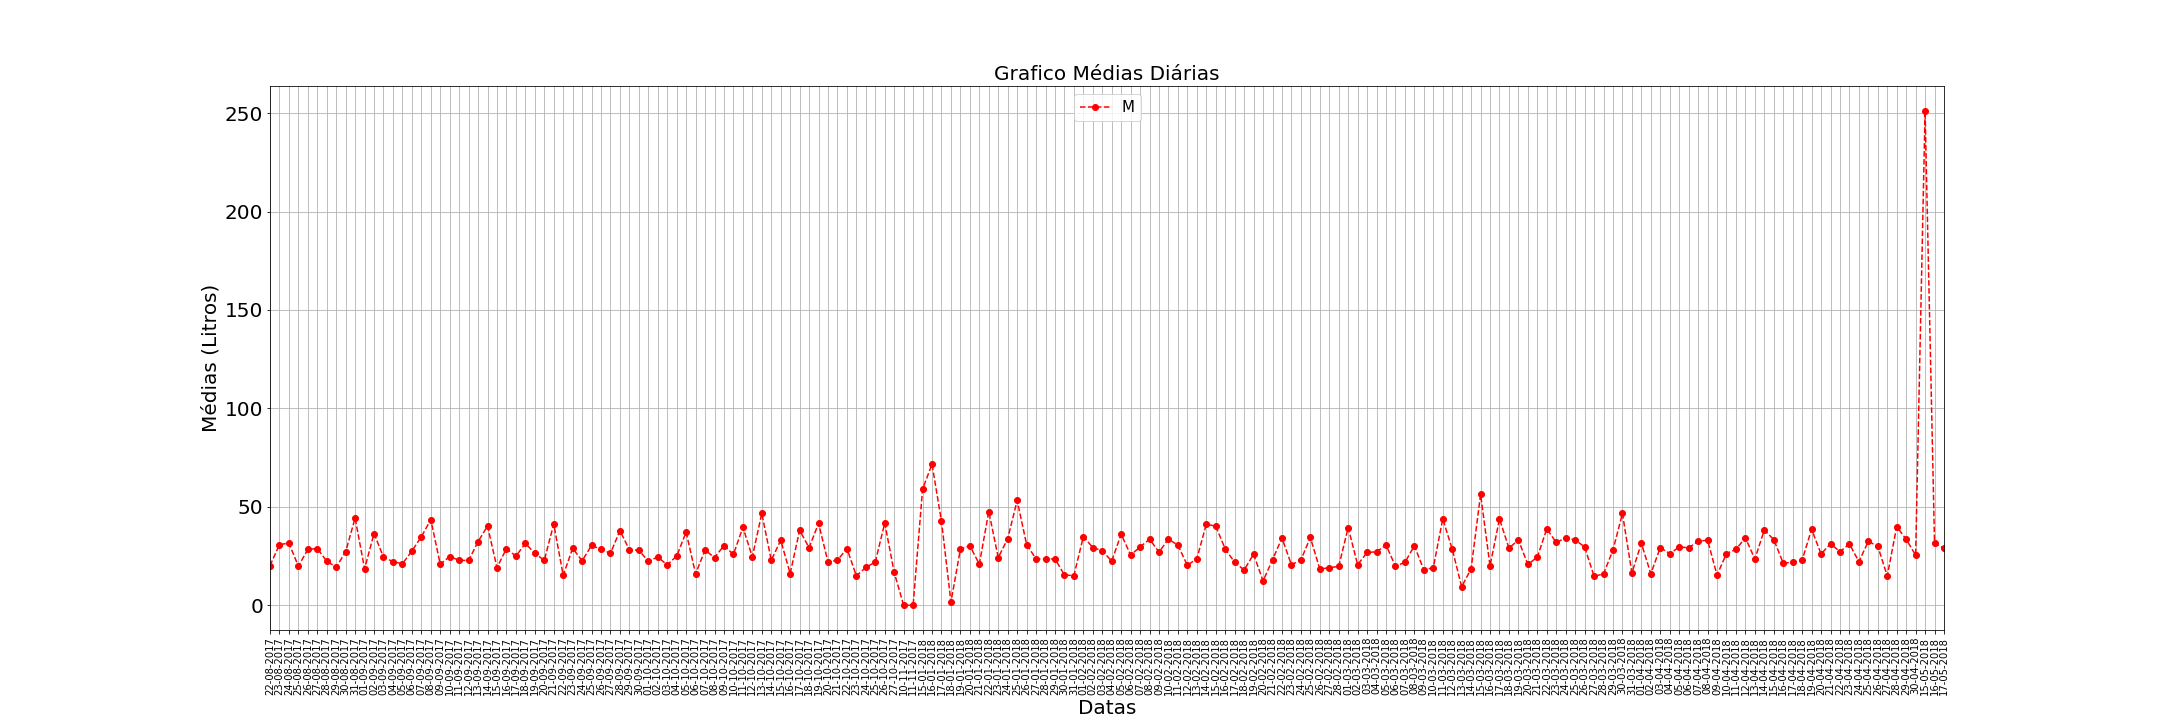
\includegraphics[width=\textwidth,height=\textheight , keepaspectratio]{figuras/GraficoMediasDiarias(este)}
		\label{graf_media_diaria}
	%\fonte{\cite{fayyad1996data}}
\end{figure}

\begin{figure}[ht]
	\caption{\textbf{Gráfico detalhado com médias diárias}}
	\centering
		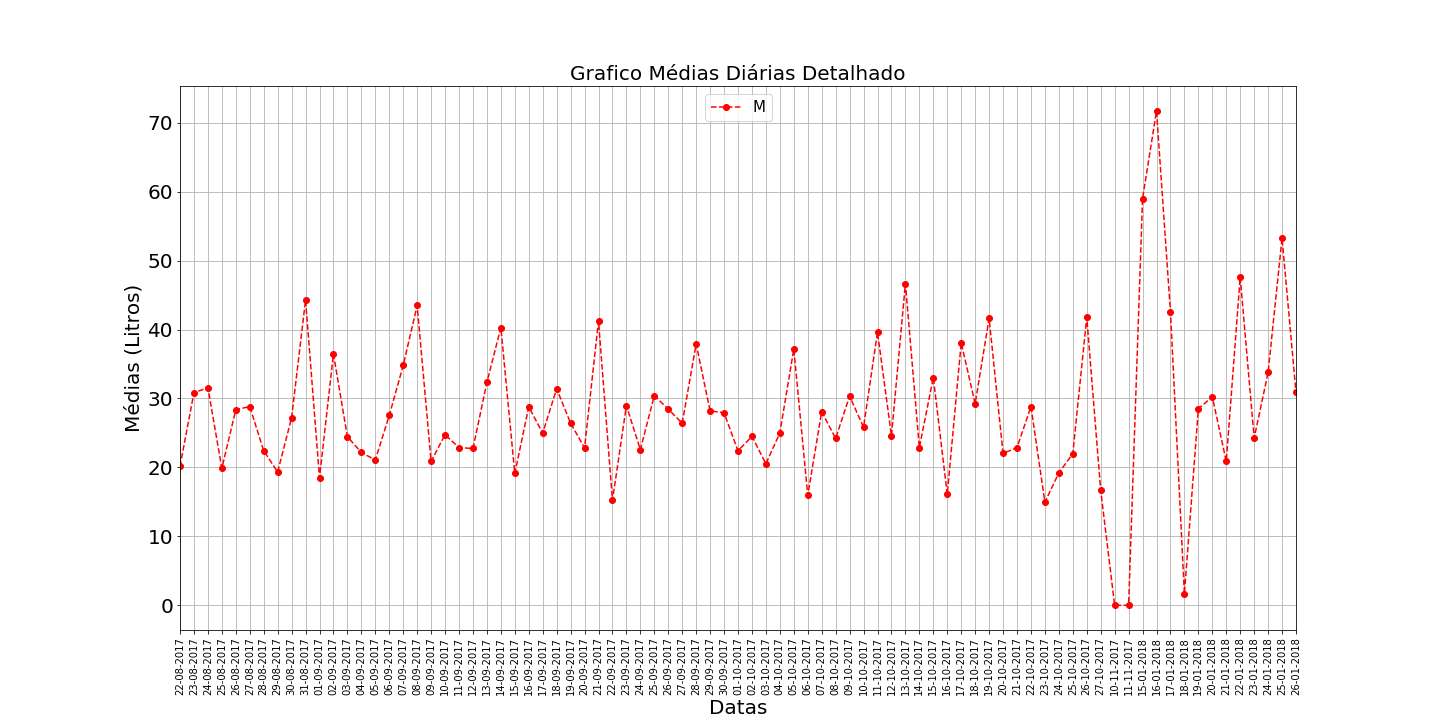
\includegraphics[width=\textwidth,height=\textheight , keepaspectratio]{figuras/GraficoMediasDiarias(estecomzoom)}
		\label{graf_media_diaria_detal}
	%\fonte{\cite{fayyad1996data}}
\end{figure}


\par Com a função detalhada na figura \ref{codigo_medias_diarias} onde foi possível realizar o cálculo das médias diárias do arquivo todo. E com a plotagem dos dados obtidos no gráfico da figura \ref{graf_media_diaria} e também no gráfico da figura \ref{graf_media_diaria_detal} sendo que este é uma plotagem dos dados mais detalhados para verificação das datas, e  observa que na maioria dos dias o consumo médio não ultrapassa 50 litros.



\begin{figure}[ht]
	\caption{\textbf{Gráfico com médias diárias dos meses setembro e outubro com Distância Euclidiana}}
	\centering
		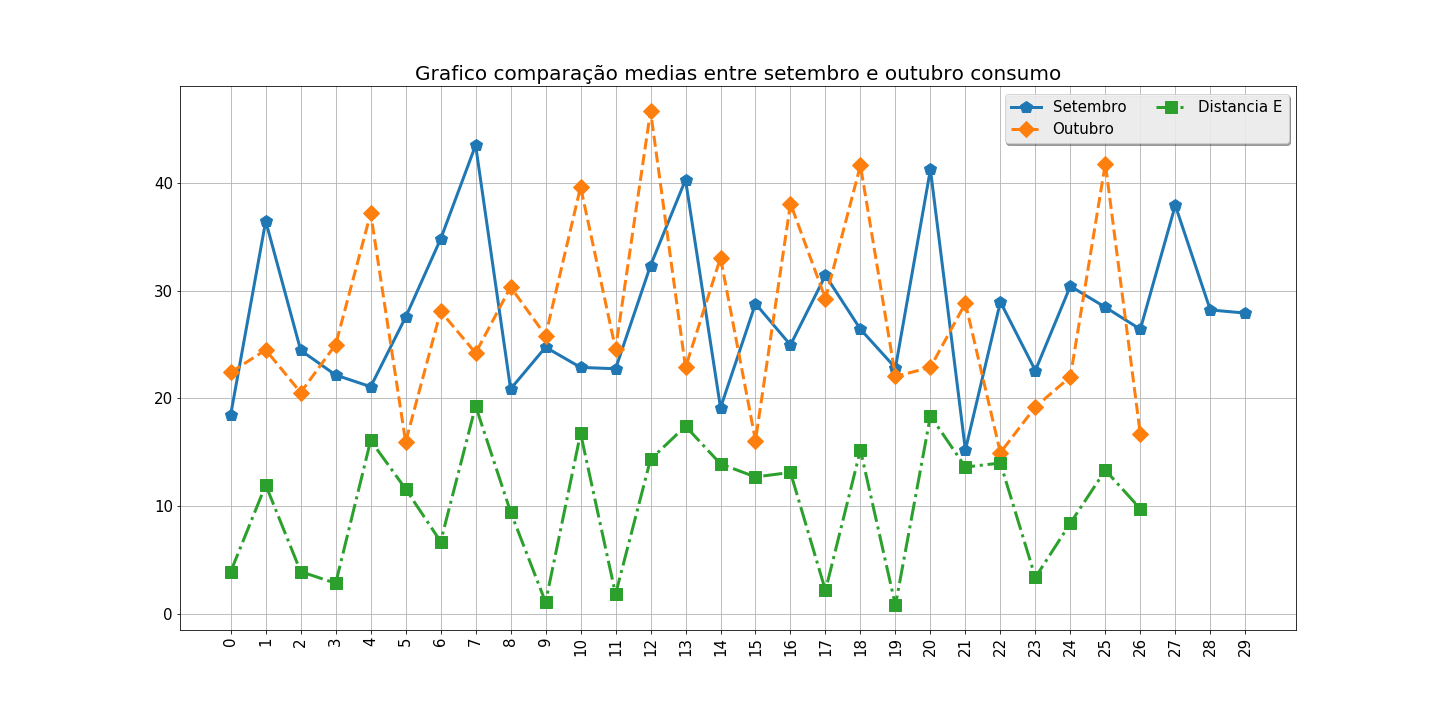
\includegraphics[width=\textwidth,height=\textheight , keepaspectratio]{figuras/comparacaomediasentredoismesesconsumocomdistanciae}
		\label{graf_media_diaria_meses_d}
	%\fonte{\cite{fayyad1996data}}
\end{figure}

\par Com o gráfico da figura \ref{graf_media_diaria_meses_d} pode se verificar a comparação das médias diárias entre os meses de setembro e outubro e junto foi realizado o cálculo com a Distância Euclidiana ponto a ponto, e em alguns pontos os resultados se aproxima de zero e observando a semelhança entre os dados.   

\begin{figure}[ht]
	\caption{\textbf{Gráfico do Total Diário de toda amostragem}}
	\centering
		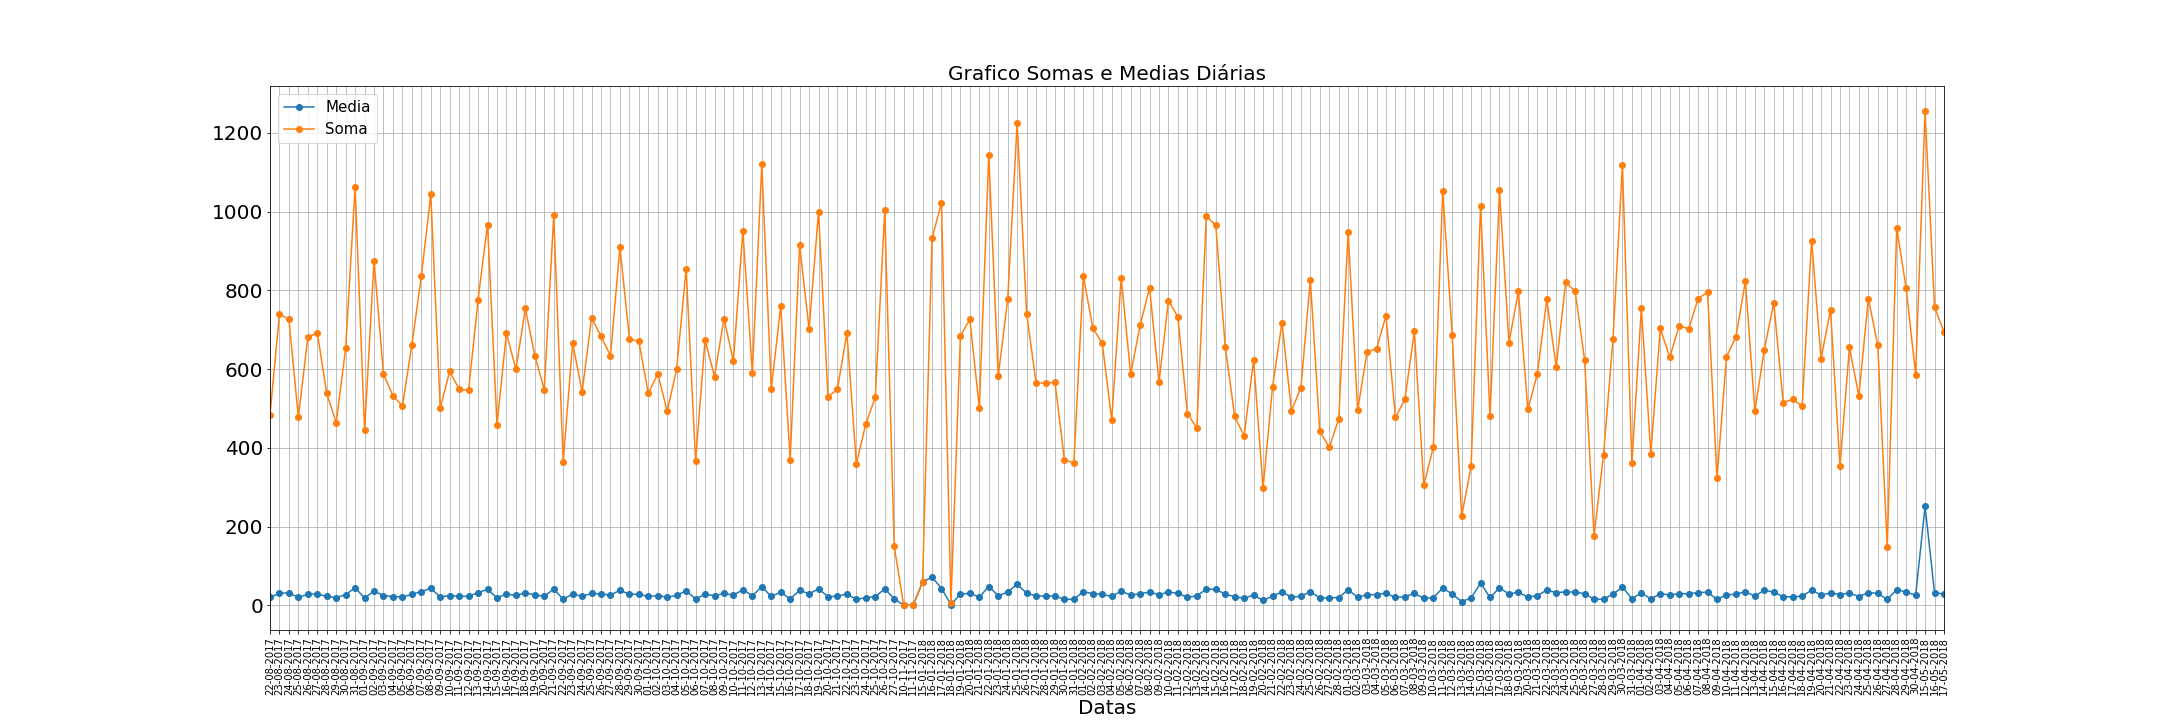
\includegraphics[width=\textwidth,height=\textheight , keepaspectratio]{figuras/GraficoSomaseMediasDiarias(este)}
		\label{graf_total_diaria}
	%\fonte{\cite{fayyad1996data}}
\end{figure}

\begin{figure}[ht]
	\caption{\textbf{Gráfico detalhado da Total Diário}}
	\centering
		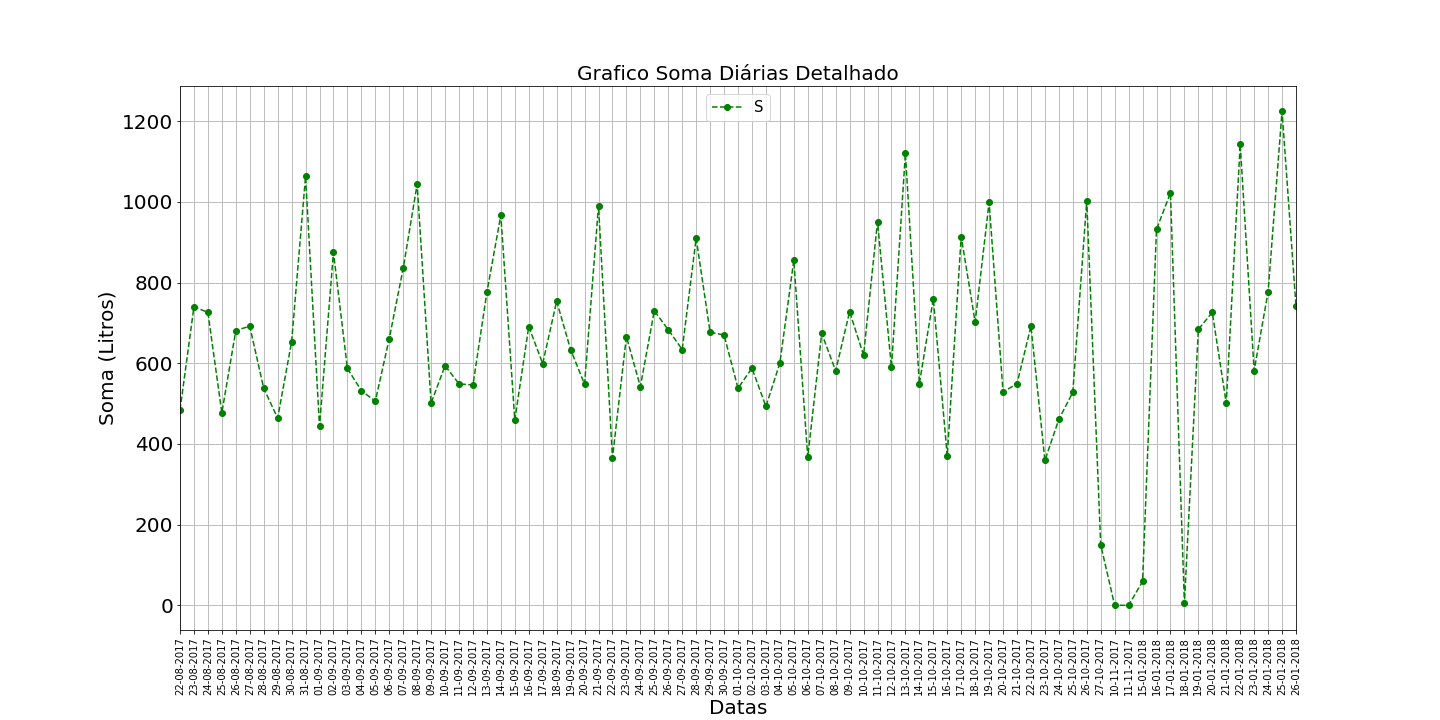
\includegraphics[width=\textwidth,height=\textheight , keepaspectratio]{figuras/GraficoSomaDiarias(estecomzoom)}
		\label{graf_total_diaria_detal}
	%\fonte{\cite{fayyad1996data}}
\end{figure}

\par Utilizando a mesma função detalhada na figura \ref{codigo_medias_diarias}, mas apenas substituindo a função \emph{“mean ()”} pela função \emph{“sum ()”}, foi possível realizar o cálculo do total diário de todo o arquivo. E com a plotagem dos dados obtidos na figura \ref{graf_total_diaria} e na figura \ref{graf_total_diaria_detal}, sendo esta uma plotagem dos dados mais detalhados para verificação, e se observa que na maioria dos dias o consumo ultrapassa 800 litros. Como já mencionado, foi constatado que nesse período dos dados não houve vazamentos, mas não pode se afirmar com certeza se houve excesso no consumo, pois teria que se fazer um estudo aprofundado obtendo o número de consumidores desse local onde foram obtidos os dados.  

\begin{figure}[ht]
	\caption{\textbf{Gráfico do Total Diário entre dois meses com Distância Euclidiana}}
	\centering
		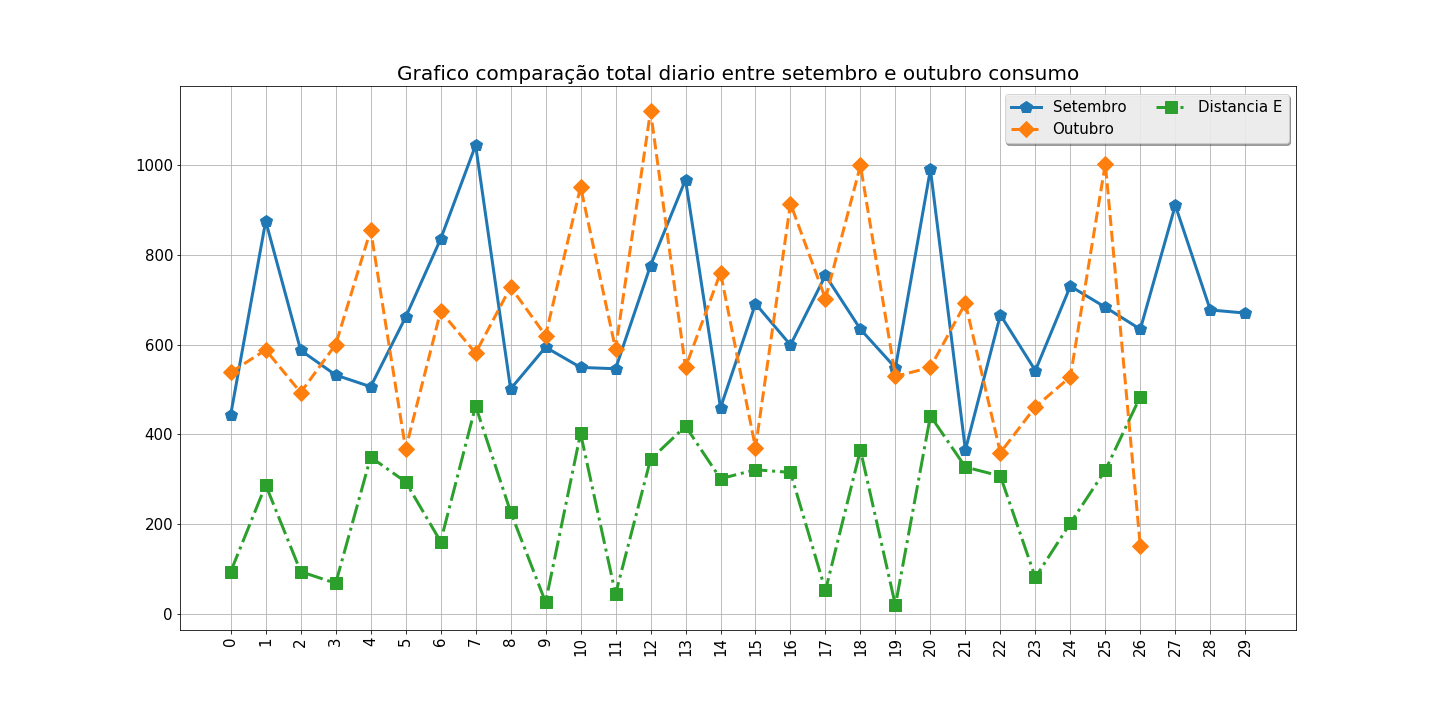
\includegraphics[width=\textwidth,height=\textheight , keepaspectratio]{figuras/comparacaototaldiarioentredoismesesconsumocomdistanciae}
		\label{graf_total_diaria_meses_d}
	%\fonte{\cite{fayyad1996data}}
\end{figure}

\par Com a figura \ref{graf_total_diaria_meses_d} pode se verificar a comparação do total diário entre os meses de setembro e outubro e junto realizado o cálculo com a Distância Euclidiana ponto a ponto e em alguns pontos os resultados se aproxima de zero e observando a semelhança entre os dados.

\begin{figure}[ht]
	\caption{\textbf{Gráfico Simulação de vazamento}}
	\centering
		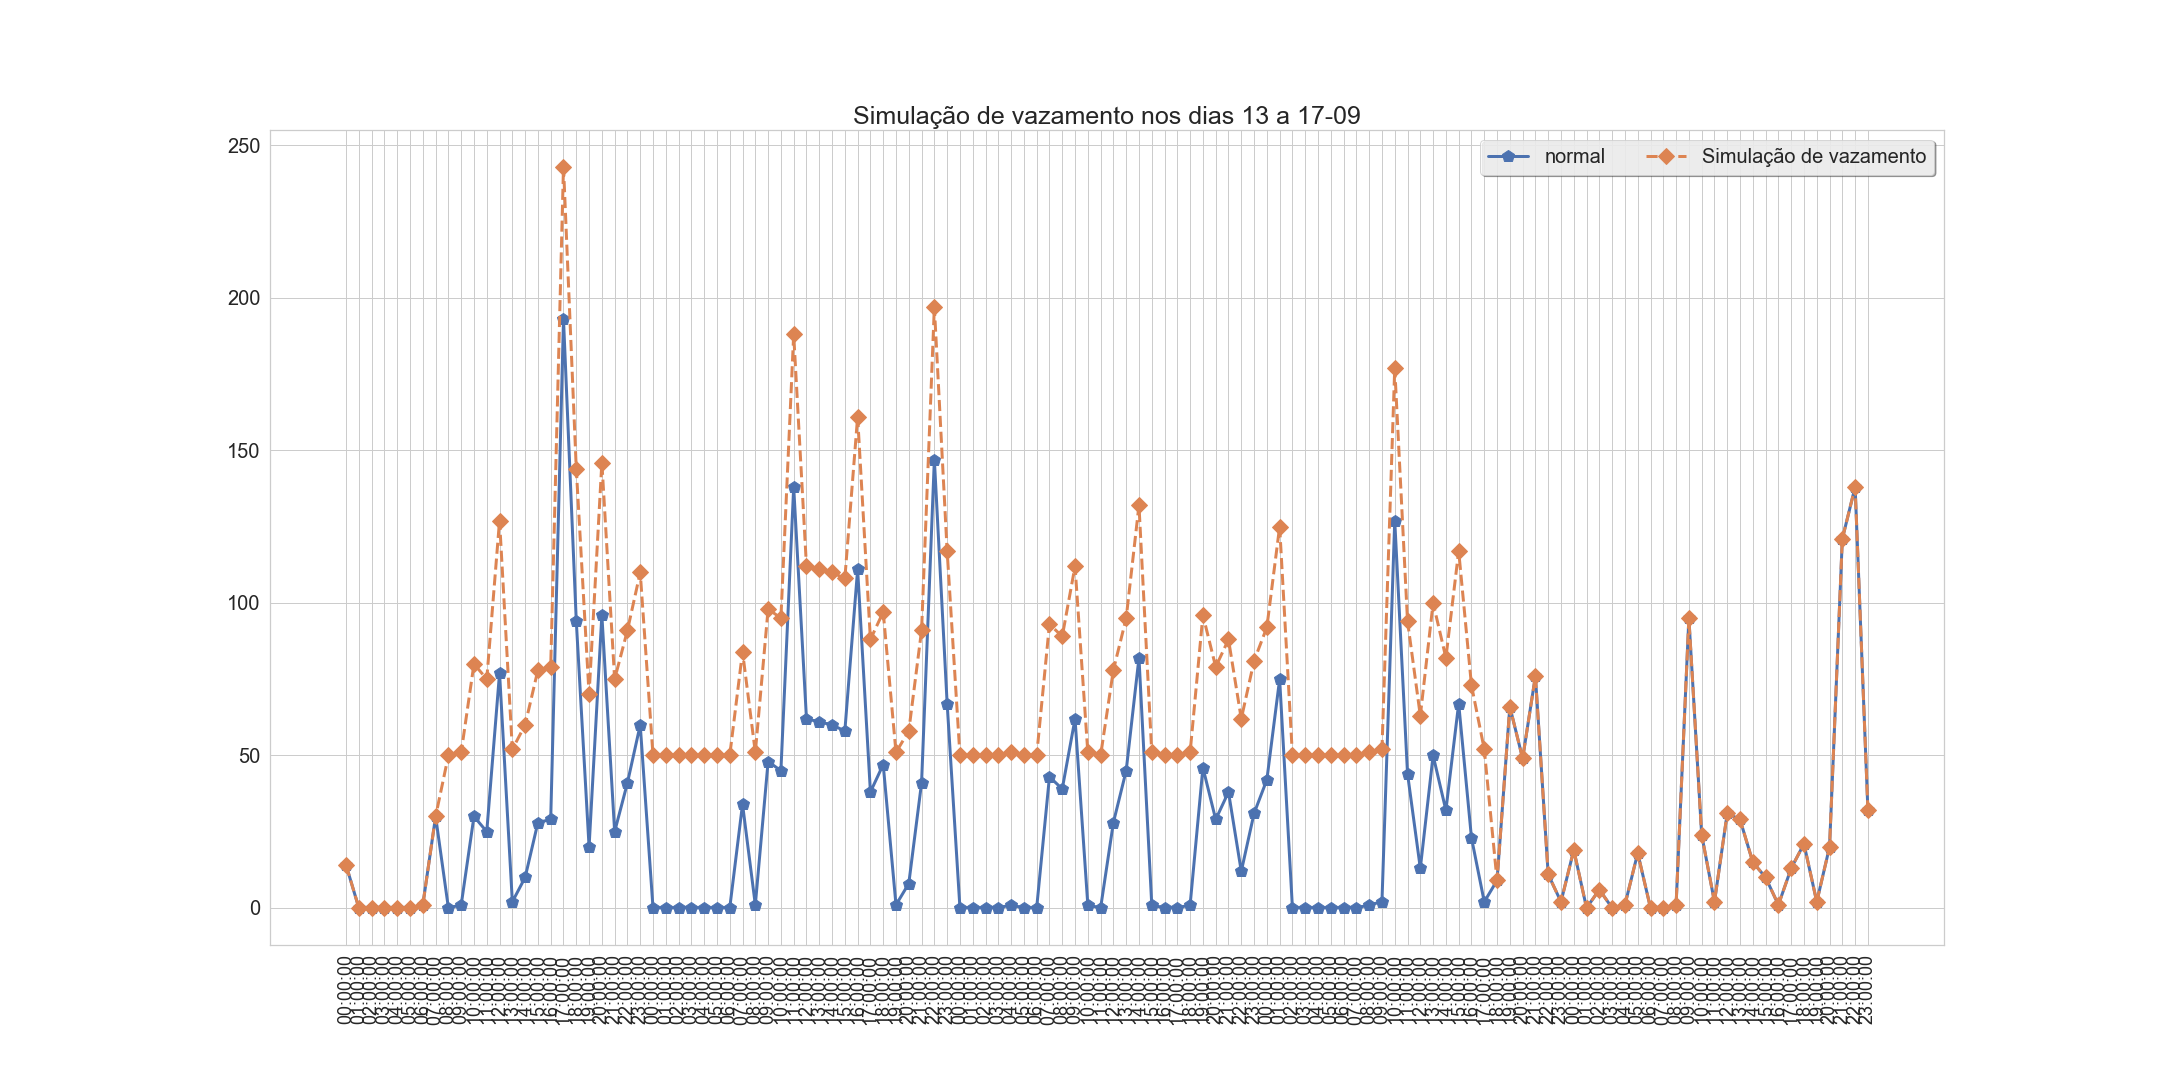
\includegraphics[width=\textwidth,height=\textheight , keepaspectratio]{figuras/Simulacaodevazamentonosdias13a17-09}
		\label{graf_simula_vaz}
	%\fonte{\cite{fayyad1996data}}
\end{figure}

\par O gráfico da figura \ref{graf_simula_vaz} é uma simulação de vazamento. Onde os dados desse mesmo mês foi acrescentada uma constante no valor 50 litros hora e aplicado o resultado desses dados no algoritmo de plotagem da figura \ref{codigo_plotagem}.  Verifica-se que continua tendo o consumo normal, mas há um aumento expressivo  por causa do vazamento. E no final após o vazamento ter sanado retorna-se ao consumo normal. E observando consumo do local onde foram extraídos os dados, o algoritmo apontou neste caso que houve um vazamento, e também apontou-nos outros casos momentos que não houve consumo e momentos onde o consumo se teve picos podendo ser ou não excesso no consumo.

\begin{figure}[ht]
	\caption{\textbf{Simulação de vazamento}}
	\centering
		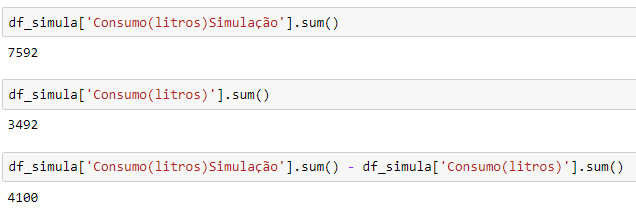
\includegraphics[width=\textwidth,height=\textheight , keepaspectratio]{figuras/somaediferencadasimulacao}
		\label{simula_vaz}
	%\fonte{\cite{fayyad1996data}}
\end{figure}

\par E com a figura \ref{simula_vaz} nota-se que o total de litros acumulados na simulação foi de 7592 litros, em comparação com o total consumido normalmente de 3492 litros, e a diferença entre a simulação e consumo normal é de 4100 litros.

\begin{figure}[ht]
	\caption{\textbf{Gráfico com a simulação de vazamento com distância euclidiana}}
	\centering
		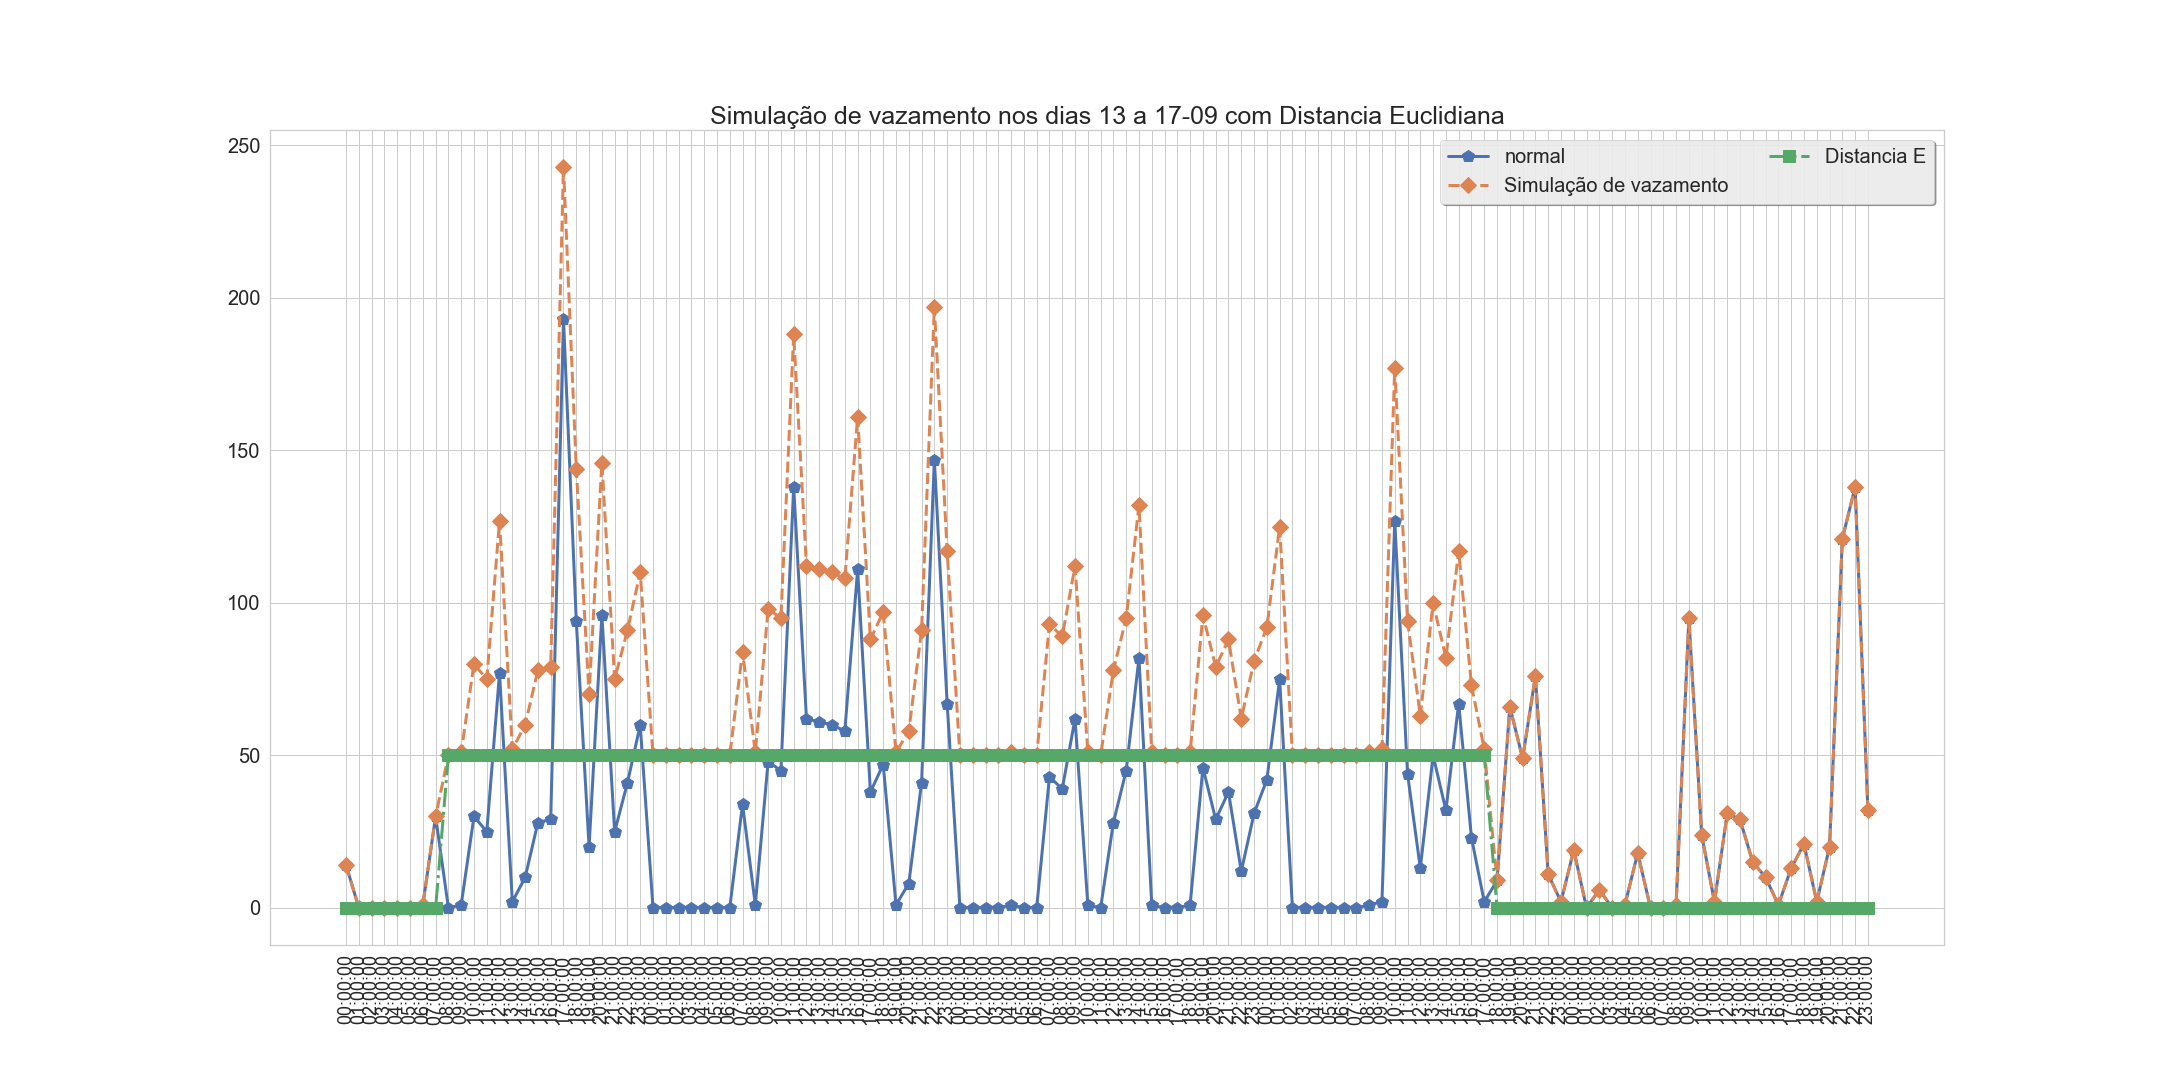
\includegraphics[width=\textwidth,height=\textheight , keepaspectratio]{figuras/Simulacaodevazamentonosdias13a17-09comDistanciaEuclidiana}
		\label{graf_simula_vaz_d}
	%\fonte{\cite{fayyad1996data}}
\end{figure}

\par A figura \ref{graf_simula_vaz_d} apresenta a mesma figura \ref{graf_simula_vaz} com uma diferença o cálculo da Distância Euclidiana ponto a ponto, pode se notar que com o cálculo houve uma ascensão dos pontos no gráfico indicando um aumento no consumo. E voltando ao estado normal assim que o problema foi sanado.

\begin{figure}[ht]
	\caption{\textbf{Gráfico da média hora a hora do arquivo todo}}
	\centering
		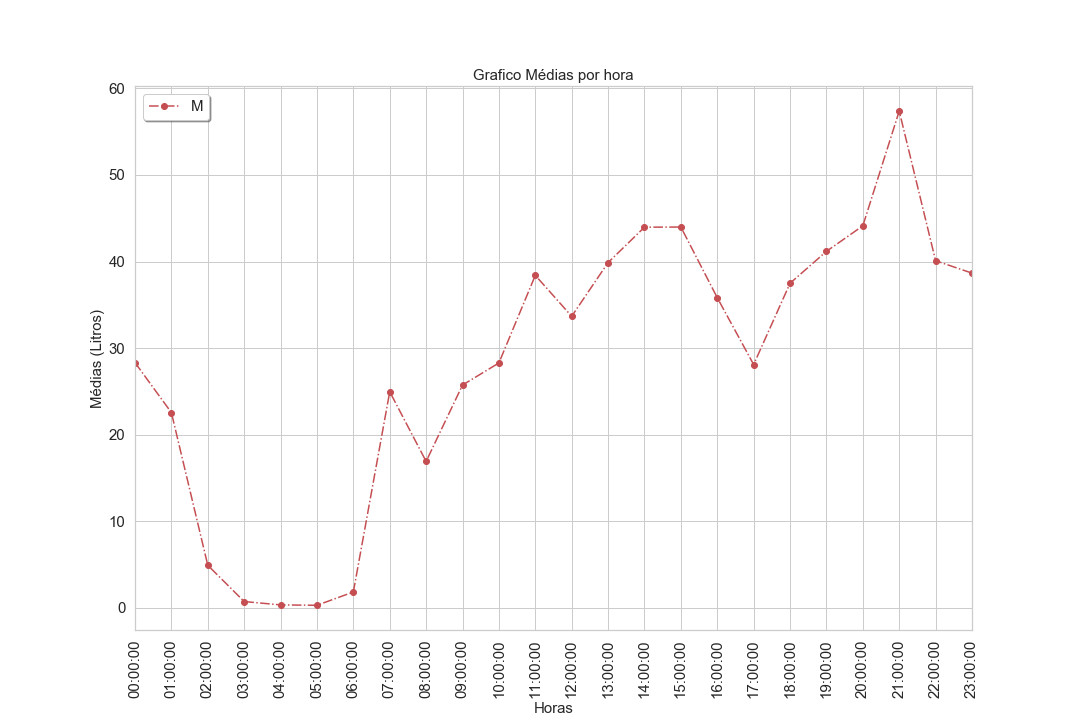
\includegraphics[width=\textwidth,height=\textheight , keepaspectratio]{figuras/GraficoMediasPorHora(este)}
		\label{graf_media_h_h}
	%\fonte{\cite{fayyad1996data}}
\end{figure}

\par Com base na função de cálculo de média, da figura \ref{codigo_medias_diarias}, foi realizada uma plotagem dos dados em gráficos com a média hora a hora total do arquivo. Como pode ser observado na figura \ref{graf_media_h_h}, com isso pode se ter uma base para estipular excesso no consumo de água. 

\begin{figure}[ht]
	\caption{\textbf{Gráfico da média hora a hora entre Fevereiro e Março e a média do arquivo todo}}
	\centering
		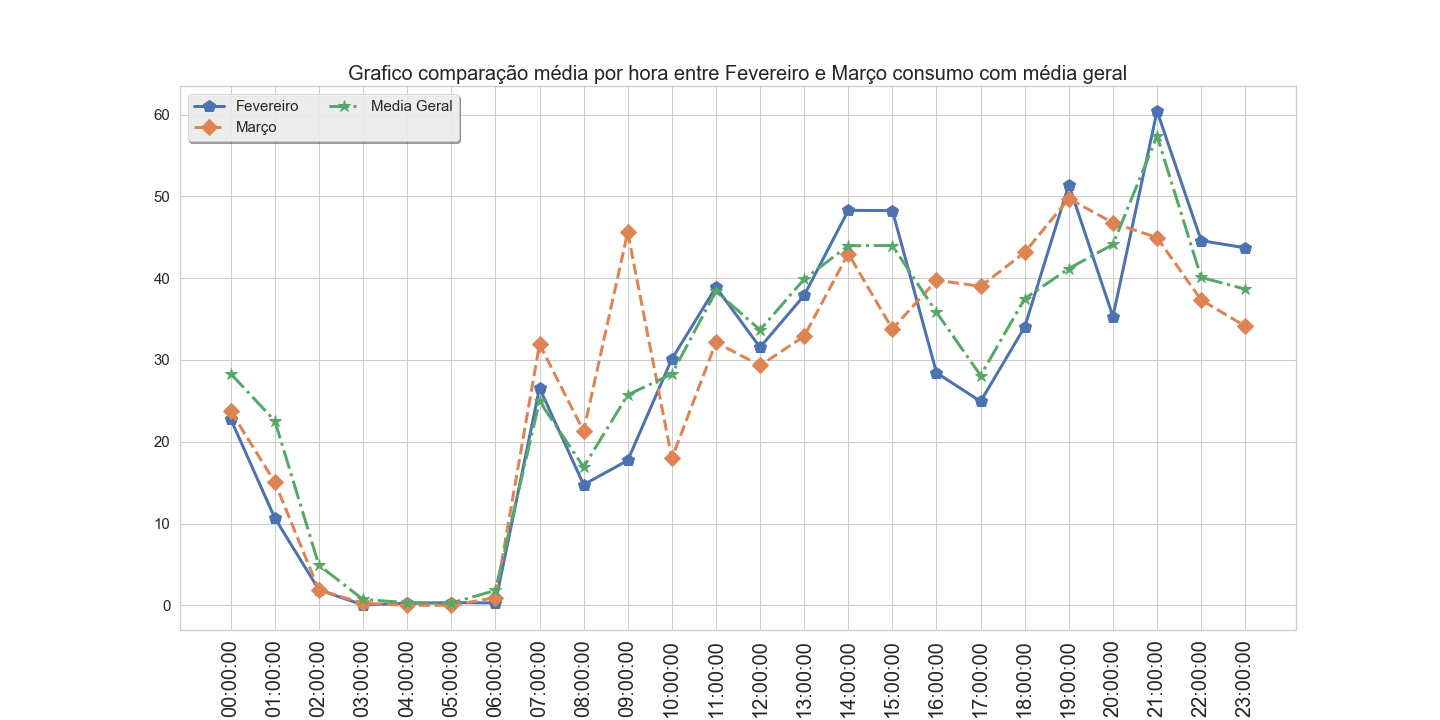
\includegraphics[width=\textwidth,height=\textheight , keepaspectratio]{figuras/comparacaomediahorarientredoismesesconsumo}
		\label{graf_media_h_h_2meses}
	%\fonte{\cite{fayyad1996data}}
\end{figure}

\par Com o gráfico da figura \ref{graf_media_h_h_2meses}, é a plotagem dos dados da comparação entre os meses de Fevereiro e Março de 2018 mais a média de todo o arquivo de dados, pode se observar há períodos semelhantes no consumo de água.

\begin{figure}[h]
	\caption{\textbf{Gráfico da média hora a hora entre Fevereiro, Março e Abril e a média do arquivo todo}}
	\centering
		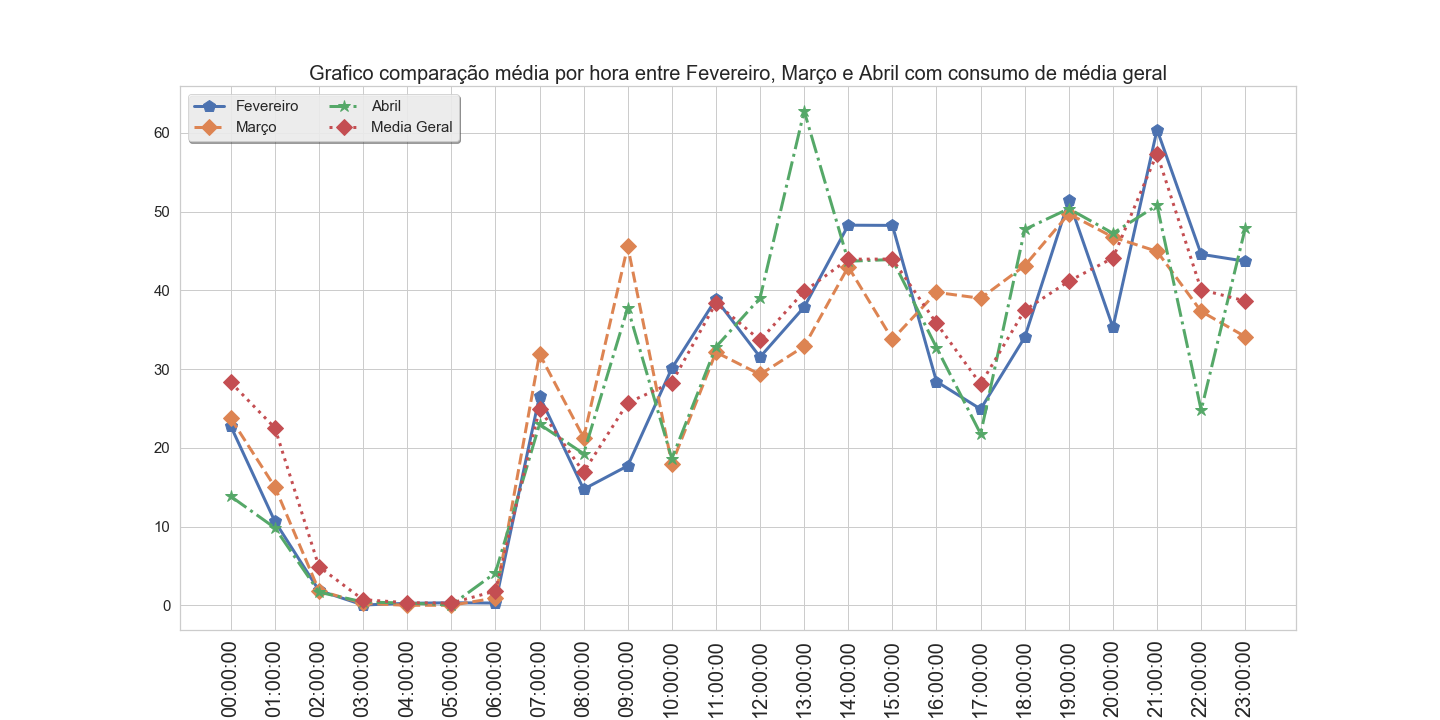
\includegraphics[width=\textwidth,height=\textheight , keepaspectratio]{figuras/comparacaomediahorarientretresmesesconsumo}
		\label{graf_media_h_h_3meses}
	%\fonte{\cite{fayyad1996data}}
\end{figure}

\par Com o gráfico da figura \ref{graf_media_h_h_3meses}, é a plotagem dos dados da comparação entre os meses de Fevereiro, Março e Abril de 2018 mais a média de todo o arquivo de dados, pode se observar há períodos semelhantes no consumo de água. 
